\graphicspath{{Figures/}}
\chapter{Robust Task-Space QP for Kinematic-Controlled Robots} \label{chap:robust qp}
%\epigraph{‘‘It is a capital mistake to theorize before one has data’’}{\emph{Arthur Conan Doyle}}
In the previous chapter, we studied the closed-loop stability in the case of  1-DoF kinematic-controlled robot. The conducted study permitted us to construct a good understanding of the source of closed instability: coupling between the task (resp. constraint) gains and the joint-dynamics parameters that leads the closed-loop system eigenvalues to be instable. Next, we proposed an integral feedback method that ensures the stability by finely tuning the integral gain.  

In this chapter, we extend the approach proposed in \cref{chap:instable qp} to the more general case: task-space QP formulation. However, this extension requires new theoretic tools and assumptions to make the approach generic enough for a larger class of kinematic-controlled robots. First, we do not restrict our formulation to joint-controllers formulated as PD and whose input is the desired position. Instead, we construct our reasoning on a simple assumption largely validated by kinematic-controlled robots: the joint-dynamics is Input-to-State-Stable (ISS) w.r.t the external disturbance torque $\jointDisturbIn$. Next, the closed-loop stability is analyzed by the robustness against non-modeled dynamics: joint-dynamics, flexibilities, etc. In addition, the proposed robust task distance-constraint formulations are proved using Lyapunov and control barrier function theories, respectively. 

In \cref{sec-chap3:QP formulation}, we formulate the task-space QP controller with the joint-dynamics model. Then, we introduce control barrier functions. Then, in \cref{sec-chap3:Robust QP}, we show how the integral feedback terms~\eqref{eq:heterogeneous feedback 1DoF closedLoop}--\eqref{eq:heterogeneous feedback constrained QP 1-DoF} in \cref{chap:instable qp} are extended to task-space QP. The synoptic view of the proposed control scheme is shown in \cref{fig:whole control scheme}. Finally, we validate the proposed QP formulation with experiments conducted on  HRP-4 humanoid robot as well as Panda robotic manipulator. 

%{\color{red}In this chapter, the subscript ‘${\rm{d}}$’ denotes the desired entity. We enhance the task-space QP formulation in~\cref{chap:adaptive gains} with the actual and desired joint/task dynamics states in \cref{sec-chap3:QP formulation}. 
%First, we will link our non-robustness observation with similar observations in the state-of-the-art works (\cref{sec-chap2:sota chap2}). Then, we start our study by considering the simple case-study: a kinematic-controlled 1-DoF robot (\cref{sec-chap2:1-DoF robot}). Even though its basic aspect, this case-study enables to understand the source of closed-loop instability. We will show how our proposed solution works for this simple example, then how we extend it to QP robust task (\cref{subsec-chap2:Robust task formulation}) and constraint (\cref{subsec-chap2:Robust constraint formulation}) formulations. To show the general applicability of our approach, experiments are conducted on a fixed-base robot and humanoid robot, both are kinematic-controlled (\cref{sec-chap2:Experiments}).
%\begin{itemize}
%	%\item {\color{OliveGreen}QP formulated in task space}
%	%\item {\color{OliveGreen}Concerning the joint-dynamics, our formulation is not specific to a specific type of joint-controllers. Instead, we construct our reasoning on a simple assumption largely validated by kinematic-controlled robots. Joint-dynamics is stable in ISS sense}
%	%\item The closed-loop robustness is studied against a larger panel of factors (not only joint-dynamics) like non-modeled flexibilities
%	%\item {\color{OliveGreen}Lyapunov and Control Barrier Function as tools to prove  task robust stability and set robust stability }
%	%\item In \cref{chap:adaptive gains}, we proved based on an analytic approach that the set $\setC$ is {\color{red}forward invariant and asymptotically stable}. This approach is not suitable to prove the robust stability of a set. Instead, we will use Control Barrier Function theory. 
%	%\item Introduce the idea of set robust stability
%	%\item Experiments shall be assessed on a robotic manipulator as well as a humanoid robot 
%	\item add section: comparison with state of the art (from paper IEEE)
%	\item search for the world ‘safety’ and replace it with stability 
%	\item modify \cref{assum1}
%	\item explain why switching to CBF in \cref{subsec-chap3:ECBF}
%\end{itemize}


%In this chapter, we will address the following question: ... 
\begin{sidewaysfigure}
	\centering
	\begin{tikzpicture}[auto, node distance=2cm,>=latex']
		\node [block](QP) {QP~\cref{eq:robust QP for combination}};
		\node [tmp, left of=QP, node distance = 6 cm] (tmpLeftQP){};
		\node [block, above of = tmpLeftQP, node distance = 0.5 cm] (Task law) {Robust Task Stabilization~\eqref{eq:heterogeneous feedback mu}};
		\node [block, below of = tmpLeftQP, node distance = 0.5 cm] (RECBF) {RECBF~\eqref{eq:RECBF formulation}};
		\node [tmp, right of=QP, node distance = 2.5 cm] (alphaD){};
		\node [block, right of=alphaD, node distance = 3 cm](integrator) {Double Integrator~\eqref{eq:double integrator}};
		\node [tmp, right of= integrator, node distance = 3.5 cm] (tmpXd){};
		\node [tmp, above of= tmpXd, node distance = 1 cm] (tmpFB){};
		\node [tmp, below of= tmpXd, node distance = 1 cm] (tmpxd){};
		\node [tmp, right of=integrator, node distance = 4 cm] (xd){};
		\node [block, right of=xd, node distance = 2 cm,pin={[pinstyle]above:$\jointDisturbIn$}](robot) {Robot~\eqref{eq:robot dynamics}};
		\node [input, above of = robot, node distance = 1cm] (tmpDisturb) {};
		\node [tmp, right of=robot, node distance = 1.5 cm](x){};
		\node [tmp, right of=x, node distance = 0.7 cm](x2){};		
		\node [block, below of = QP, node distance = 3 cm, text width=4cm] (forward kin and vel task) {Forward Kinematics \&  Forward Velocity~\eqref{eq:act output vector}};
		\node [block, below of = forward kin and vel task, node distance = 1.7 cm, text width=4cm, thick, draw = blue] (forward vel task) {Forward Velocity~\eqref{eq:des output vector}};
		\node [dotted_block, fit = (forward kin and vel task) (forward vel task)] (task) {};		
		\node at (task.north) [above, inner sep=1.0mm] {Task States};
		
		\node [block, below of = forward vel task, node distance = 3 cm, text width=4cm] (forward kin and vel constr) {Forward Kinematics \&  Forward Velocity~\eqref{eq:act Bfunc state}};
		\node [block, below of = forward kin and vel constr, node distance = 1.7 cm, text width=4cm, thick, draw = blue] (forward vel constr) {Forward Velocity~\eqref{eq:des Bfunc state}};
		\node [dotted_block, fit = (forward kin and vel constr) (forward vel constr)] (constr) {};		
		\node at (constr.north) [above, inner sep=1.0mm] {Distance-Constraint States};
		
		\node [block, left of = forward kin and vel task, node distance = 4 cm] (K task) {$\taskGains$};
		\node [block, left of = forward vel task, node distance = 4 cm, thick, draw = blue] (Lv task) {$\taskIntegralDamping$};
		\node [block, left of = forward kin and vel constr, node distance = 4 cm] (K constr) {$\constraintGains$};
		\node [block, left of = forward vel constr, node distance = 4 cm, thick, draw = blue] (Lv constr) {$\constraintIntegralDamping$};
		
		\node [tmp, left of = Task law, node distance = 4cm] (tmpLeftTask) {};
		\node [tmp, left of = RECBF, node distance = 4cm] (tmpLeftConstr) {};
		
		%\fill [rotate=0] (4.85,-.5)rectangle(4.5,.5);
		\draw [line width=2pt](9,-.5)--(9,.5);
		\draw [->] ([yshift=0.2cm] tmpXd) -| node[above,yshift = 0.1cm, pos=0.85]  {$\desFBDyn$}([xshift = 0.3 cm]tmpFB);
		\draw [-] ([yshift=-0.2cm] tmpXd) -- ([yshift=-0.2cm, xshift=0.5cm] tmpXd);%([xshift = 0.5 cm]tmpxd);
		\draw [->] ([yshift=-0.2cm, xshift=0.5cm] tmpXd) |- node[near end] {$\desJointDyn$} (robot.west);
		%	\node [tmp, right of=robt, node distance = 2 cm](x){};
		\node [tmp, below of = QP, node distance = 0.5cm] (aux){};
		%	\draw [->] (u) -- node{$\jointCrtlIn$}(xd dynamics);
		\draw [->] (QP) -- node{$\UgenDesJointDyn$}(integrator);
		%	\draw [->] (tmpXd) -- node{$\desJointDyn$}(robot);
		\draw [-|] (integrator) -- node{$\genDesJointDyn$}(tmpXd);
		%\draw [->] (tmpDisturb) -- node[pos=0]{$\jointDisturbIn$}(robot);
		%	\draw [-] (xd) |- (aux);
		\draw [->] (robot) -- node[pos=0.7]{$\genActJointDyn$}(x2);
		\draw [->] (forward kin and vel task) -- node[pos=0.7, above]{$\actTaskOut$}(K task);
		\draw [->, thick, color=blue] (forward vel task) -- node[pos=0.7, above]{${\desTaskOut}_2$}(Lv task);
		\draw [->] (forward kin and vel constr) -- node[pos=0.7, above]{$\actBfuncOut$}(K constr);
		\draw [->, thick, color=blue] (forward vel constr) -- node[pos=0.7, above]{$\desBfuncOut_2$}(Lv constr);
		
		\draw [->] ([xshift=-0.5cm]x2) |- (forward kin and vel task.east);
		\draw [->] ([xshift=-0.5cm]x2) |- (forward kin and vel constr.east);
		\draw [->, thick, color=blue] ([xshift=-0.25cm]tmpXd) |- (forward vel task.east);
		\draw [->, thick, color=blue] ([xshift=-0.25cm]tmpXd) |- (forward vel constr.east);
		
		\draw [-] (K task) -| node[pos=0.15, above]{$\taskGains\actTaskOut$}([yshift=3pt]tmpLeftTask);
		\draw [-, thick, color=blue] (Lv task) -| node[pos=0.15, above]{$\taskIntegralDamping{\desTaskOut}_2$}([yshift=-3pt,xshift = 7 pt]tmpLeftTask);
		\draw [-] (K constr) -| node[pos=0.15, above]{$\constraintGains\actBfuncOut$}([yshift=3pt,xshift = 20 pt]tmpLeftConstr);
		\draw [-, thick, color=blue] (Lv constr) -| node[pos=0.15, above]{$\constraintIntegralDamping\desBfuncOut_2$}([yshift=-3pt,xshift = 27 pt]tmpLeftConstr);
		
		\draw [->] ([yshift=3pt]tmpLeftTask) -- ([yshift=3pt]Task law.west);
		\draw [->, thick, color=blue] ([yshift=-3pt,xshift = 7 pt]tmpLeftTask) -- ([yshift=-3pt]Task law.west);
		\draw [->] ([yshift=3pt,xshift = 20 pt]tmpLeftConstr) -- ([yshift=3pt]RECBF.west);
		\draw [->, thick, color=blue] ([yshift=-3pt,xshift = 27 pt]tmpLeftConstr) -- ([yshift=-3pt]RECBF.west);
		\draw [-] (Task law.east) -- ([xshift = 10pt]Task law.east);
		\draw [-] (RECBF.east) -- ([xshift = 44pt]RECBF.east);
		\draw [->] ([xshift = 10pt]Task law.east) |- node[pos=0.8, above]{$\taskCrtlIn$}([yshift = 3pt]QP.west);
		\draw [->] ([xshift = 44pt]RECBF.east) |- node[pos=0.8, below]{$\bfuncCrtlIn$}([yshift = -3pt]QP.west);
		%	\draw [->] (disturbance) --node{$\jointDisturbIn$} (x dynamics.north);
	\end{tikzpicture}
	\caption{Overview of the proposed robust QP control scheme. The thick blue paths show the high-level integral feedback. Note that if $\taskIntegralDamping=0$ and $\constraintIntegralDamping=0$, correspond to the feedback control scheme in~\cref{subfig:feedback QP}.}
	\label{fig:whole control scheme}
\end{sidewaysfigure}
%\end{landscape}

\section{Task-Space QP Control Formulation}\label{sec-chap3:QP formulation}
\subsection{Joint-Dynamics}\label{subsec-chap3:in-out joint dynamics}
Following from~\cref{eq-chap0:gen act conf def},
let $\genActJointDyn,\genDesJointDyn\in\mathbb{R}^{13+2n}$ defined as
\begin{equation}\label{eq:gen joint dyn def}
	\genActJointDyn^T = \begin{bmatrix}
		\genActConf^T & \genActConfDot^T
	\end{bmatrix}, \	\genDesJointDyn^T = \begin{bmatrix}
		\genDesConf^T & \genDesConfDot^T
	\end{bmatrix},
\end{equation}
be the actual and desired robot states, respectively. Let $\desJointDyn,\actJointDyn\in\mathbb{R}^{2n}$ defined as
\begin{equation}\label{eq:actuated DoF states}
	\actJointDyn^T = \begin{bmatrix}
		\actConf^T & \actConfDot^T
	\end{bmatrix}, \	\desJointDyn^T = \begin{bmatrix}
		\desConf^T & \desConfDot^T
	\end{bmatrix},
\end{equation} be the actual and desired states of the robot actuated DoF. Let us define  $\jointTrackErr$ as %be the joint-dynamics tracking error defined as 
\begin{align}\label{eq:joint tracking error}
\begin{split}
	\jointTrackErr &= \genActJointDyn - \genDesJointDyn \\
	&= \begin{bmatrix}
		\FB - \desFB \\
		\actConf  - \desConf \\ 
		\FBDot - \desFBDot \\
		\actConfDot - \desConfDot
	\end{bmatrix}\inR^{13+2n} ,
\end{split}	
\end{align}
where $\FB - \desFB = \begin{bmatrix}
\bm{p}^{\rm FB} - \bm{p}^{\rm FB}_{\rm d} \\ 
\quaternion^{\rm FB} \otimes{\quaternion^{\rm FB}_{\rm d}}^{-1}
\end{bmatrix}\inR^7$ encompasses the Cartesian coordinates and orientation differences between $\FB$ and $\desFB$ (please, refer to \cref{sec-app:quaternion product}). In particular, let us define the joint-dynamics tracking error $\jointDynTrackErr$ as %be the joint-dynamics tracking error defined as 
\begin{align}\label{eq:jointDyn tracking error}
	\begin{split}
		\jointDynTrackErr = \actJointDyn - \desJointDyn\inR^{2n}.
	\end{split}	
\end{align} 
$\genDesJointDyn$ and $\genActJointDyn$ dynamics are defined as
\begin{align}\label{eq:double integrator}
	\genDesJointDynDot &=
	\begin{bmatrix}
		\mathbf{0} & \mathbf{I}_{6+n} \\
		\mathbf{0} & \mathbf{0}
	\end{bmatrix}
	\genDesJointDyn + 
	\begin{bmatrix}
		\mathbf{0} \\
		\mathbf{I}_{6+n}
	\end{bmatrix} \UgenDesJointDyn, \ \UgenDesJointDyn = \begin{bmatrix}
		\FBCrtlIn \\ \jointCrtlIn
	\end{bmatrix}, \\
	\label{eq:robot dynamics}\genActJointDynDot &= \begin{bmatrix}
		\genActConfDot\\ \genActConfDDot
	\end{bmatrix},
\end{align}
with  $\UgenDesJointDyn\in {\cal U}$ where ${\cal U}\subseteq\mathbb{R}^{6+n}$ is the set of $\UgenDesJointDyn$ admissible values, $\FBCrtlIn=\desFBDDot\in\mathbb{R}^6$ is the desired floating-base (linear and angular) acceleration,  $\jointCrtlIn \in\ \mathbb{R}^n$ is the desired joint acceleration.   	The actual floating-base state ${\actFBDyn}\tp=\begin{bmatrix}
	{\FB}\tp & {\FBDot}\tp
\end{bmatrix}\in \mathbb{R}^{13}$ 
is assumed to be bounded and estimated by an observer. From~\cref{eq:double integrator}, $\genDesJointDyn$ follows a double integrator dynamics. More importantly, given a kinematic-controlled robot, the actual robot state is governed  by the joint-dynamics\footnote{For the sake of generality, both $\desConf$ or $\desConfDot$ (joint commands) are encompassed by $\desJointDyn$ in the joint-dynamics $f_{\jointDynTrackErr}$ in \cref{eq:joint-dynamics}.} defined as 
\begin{equation}\label{eq:joint-dynamics}
\jointDynTrackErrDot = f_{\jointDynTrackErr}(\jointDynTrackErr,\jointDisturbIn),
\end{equation}   
where  $\jointDisturbIn\in\mathbb{R}^n$ is the bounded joint-space disturbance torque input. In this study, we consider that $f_{\jointDynTrackErr}$ is not known exactly but its main property is given by the following assumption.
\begin{assumption}\label{assum1}
	The joint-dynamics $f_{\jointDynTrackErr}$ in~\cref{eq:joint-dynamics} is globally asymptotically stable at the origin for $\jointDisturbIn=\bm{0}$, and ISS w.r.t  $\jointDisturbIn\neq0$.
\end{assumption}%\footnote{System~\cref{eq:low level system 2} is then said to be \emph{fully stable} according to Definition 10 in~\cite{andriano1997nonlinearAnalysis}.}. 
%IS-Stability is the generalization of Bounded-Input-Bounded-State stability for nonlinear systems. 
The IS-Stability ensures that, given  bounded disturbance inputs $\jointDisturbIn$,  the joint-dynamics tracking error $\jointTrackErr$ evolves in a bounded set containing the origin (see formal definition in \cref{ann:ISS}).	
\cref{assum1} is largely valid as it is among the main requirement for the well-functioning of a kinematic-controlled robot.

%Let us define  $\jointTrackErr$ as %be the joint-dynamics tracking error defined as 
%\begin{align}\label{eq:joint tracking error}
%	\begin{split}
%		\jointTrackErr &= \genActJointDyn - \genDesJointDyn \\
%					   &= \begin{bmatrix}
%					   	\FB - \desFB \\
%					   	\actConf  - \desConf \\ 
%					   	\FBDot - \desFBDot \\
%					   	\actConfDot - \desConfDot
%					   \end{bmatrix}\inR^{13+2n} ,
%	\end{split}	
%\end{align}
%where $\FB - \desFB = \begin{bmatrix}
%	\trans(\FB) - \trans(\desFB) \\ 
%	\quat(\FB) \otimes \quat(\desFB)^{-1}
%\end{bmatrix}\inR^6$ encompasses the Cartesian coordinates and orientation differences between $\FB$ and $\desFB$ (please, refer to \cref{sec-app:quaternion product}).
$\jointTrackErr$ in \cref{eq:joint tracking error} reflects the effect of several kind of disturbances and uncertainties. Namely, non-modeled dynamics (e.g., transient joint-dynamics response w.r.t $\desJointDyn$, flexibilities, etc.); hardware imperfections (e.g., joint-dynamics steady-state errors, etc.); external disturbance $\jointDisturbIn\neq0$ (e.g., pushes, unexpected impacts, etc.); measurement and  estimation noises (joint-velocity and floating-base estimations, etc.); and possibly others\footnote{A benchmark problem has been proposed in~\cite{moberg2009tcst} that simulates such disturbances.}.
\begin{remark}\label{rem:fixed-base robot case}
	For a fixed-base robot, we have $\genActConf=\actConf$ and  $\UgenDesJointDyn = \jointCrtlIn$ which implies that $\genActJointDyn = \actJointDyn$ (and respectively for the corresponding desired states).
\end{remark}
%\emph{Remark~\showmycounter{rem1}:} 
	



\subsection{Input-Output Task Dynamics}\label{subsec-chap3:in-out task dynamics}
Let  $\fkin:\mathbb{R}^{7+n} \rightarrow\mathbb{R}^m$ be the forward kinematics of a given task defined by $m$ coordinates, and $\fkinRef(t),\fkinRefDot(t),\fkinRefDDot(t)\in\mathbb{R}^m$ be the task references. % assumed to be twice differentiable. 
%	Let be $\desOut\!=\!\fkin(\genDesConf)\! -\! \fkinRef$ and $\actOut\!=\!\fkin(\genActConf) \!-\! \fkinRef$ be the desired and actual task outputs, such that $\desOut\!=\!\text{col}(\desOut^i)$, $i \!=\!1,\dots, m$ where each $\desOut^i \!\in\!\mathbb{R}$ has a relative degree of 2
%	\begin{equation*}
	%		\desOutDDot^i =  \desJac^i\UgenDesJointDyn + \desJacDot^i\genDesConfDot %- \fkinRefDDot^i(t)
	%	\end{equation*}  
Thus, we can define the following states
\begin{align}
	\label{eq:des output vector}
	\desTaskOut(\genDesJointDyn) &\!=\! 	\begin{bmatrix}
		\desTaskOutOne \\ % {\desTaskOut}_1 \\
		\desTaskOutTwo %{\desTaskOut}_2
	\end{bmatrix}=
	\begin{bmatrix}
		\desOut \\
		\desOutDot
	\end{bmatrix}=
	\begin{bmatrix}
		\fkin(\genDesConf) - \fkinRef(t) \\
		\desJac\genDesConfDot - \fkinRefDot(t) %AK> pourquoi ne pas considérer le cas general du tracking, donc on gardant \fkinRefDot?
	\end{bmatrix}\in H^{\fkin}\subset\mathbb{R}^{2m} %\\
\end{align}
\begin{align}
	\label{eq:act output vector}
	\actTaskOut(\genActJointDyn) &= \begin{bmatrix}
		\actTaskOutOne \\ %_1 \\
		\actTaskOutTwo%_2
	\end{bmatrix}=
	\begin{bmatrix}
		\actOut \\
		\actOutDot
	\end{bmatrix} =
	\begin{bmatrix}
		\fkin(\genActConf) - \fkinRef(t) \\
		\actJac\genActConfDot - \fkinRefDot(t)
	\end{bmatrix} \in H^{\fkin}\subset\mathbb{R}^{2m}
\end{align}
where $\desJac,\actJac\in\mathbb{R}^{m\times(6+n)}$ are the task Jacobians computed w.r.t $\genDesConf$ and $\genActConf$, respectively; $\desTaskOut(\genDesJointDyn)$ and $\actTaskOut(\genActJointDyn)$ denote the desired and actual task dynamics states, respectively. 
Using Taylor expansion and~\cref{eq:joint tracking error}, a relation between $\actTaskOut$ and $\desTaskOut$ is obtained as
\begin{align}\label{eq:DL act task}
	\begin{split}
		\actTaskOut(\genActJointDyn) &= \actTaskOut(\genDesJointDyn+\jointTrackErr)\\ 	
		&= \left.\begin{matrix}\actTaskOut(\genActJointDyn)\end{matrix}\right|_{\genActJointDyn=\genDesJointDyn} + \underset{\taskTrackErr}{\underbrace{\left.\begin{matrix} \frac{\partial\actTaskOut(\genActJointDyn)}{\partial\genActJointDyn}\end{matrix}\right|_{\genActJointDyn=\check{\genActJointDyn}}\jointTrackErr}}, \ \check{\genActJointDyn} = \genDesJointDyn + \theta\jointTrackErr\\
		&=\desTaskOut(\genDesJointDyn) +\taskTrackErr,\ \frac{\partial\actTaskOut(\genActJointDyn)}{\partial\genActJointDyn} = 
		\begin{bmatrix}
			\actJac & \bm{0} \\ \frac{\partial\left(\actJac\genActConfDot\right)}{\genActConf} & \actJac
		\end{bmatrix} 				
	\end{split}
\end{align} with $0\leq\theta\leq1$ and $\taskTrackErr\inR^m$ being the Lagrange remainder of  Taylor expansion and  denotes the mapping of $\jointTrackErr$ in task-space. Hereafter, the dependency of $\desTaskOut$ and $\actTaskOut$ on $\genDesJointDyn$ and $\genActJointDyn$, respectively, is dropped.
\begin{remark}\label{rem:phi orientation consideration}
	In the multiplication $\left.\begin{matrix} \frac{\partial\actTaskOut(\genActJointDyn)}{\partial\genActJointDyn}\end{matrix}\right|_{\genActJointDyn=\check{\genActJointDyn}}\jointTrackErr$, only the vector part of $\quaternion^{\rm FB} \otimes{\quaternion^{\rm FB}_{\rm d}}^{-1}$ is considered.  
\end{remark}
%\begin{remark} 
%	The orientation part of the sum  $\desJointDyn + \jointTrackErr $ is obtained by the following quaternion multiplication 
%	\begin{equation}
%		\quat(\FB) \otimes \quat(\desFB) \otimes \quat(\desFB)^{-1} = \quat(\FB)
%	\end{equation}
%\end{remark}
Given that $\desOut$ in~\cref{eq:des output vector} has a relative-degree of 2
\begin{equation}\label{eq:task relative degree}
	\desOutDDot=  \desJacDot\genDesConfDot + \desJac \UgenDesJointDyn -\fkinRefDDot(t),
\end{equation} 
then, the input-output task dynamics is obtained such that
\begin{align}\label{eq:des task dyn}
	\desTaskOutDot &= \AdesTaskOut\desTaskOut + \BdesTaskOut\taskCrtlIn \\ \label{eq:zero dyn}
	\zeroDynDot &=f_{\zeroDyn}(\zeroDyn,\desTaskOut)\\
	%	\end{align}
%	with
%	\begin{align}
	%	\begin{split}
		\AdesTaskOut &= \begin{bmatrix}
			\mathbf{0} & \mathbf{I}_m \\ \mathbf{0} & \mathbf{0}
		\end{bmatrix}, \BdesTaskOut = \begin{bmatrix}
			\mathbf{0} \\ \mathbf{I}_m
		\end{bmatrix} \\\label{eq:mapping mu to u}
		\taskCrtlIn &= \desJacDot\genDesConfDot + \desJac \UgenDesJointDyn -\fkinRefDDot(t)% \jointCrtlIn
		%	\end{split}
\end{align}
where $\zeroDyn\in Z\subset\mathbb{R}^{13+2n-2m}$ is called the internal-dynamics state as it is not observable from $\desTaskOut$~\cite{slotine1991applied}, and denotes the remaining redundancies~\cite{varghese1990icse,varghese1991taes}. Considering that $\desTaskOut$ is the input, one important assumption is that the internal dynamics~\cref{eq:zero dyn} is assumed to be ISS~\cite{isidori2013ejc}\footnote{This implies implicitly that the zero dynamics $\zeroDynDot=f_{\zeroDyn}(\zeroDyn,0)$ is asymptotically stable.}. In Section~\ref{subsec-chap3:Robust QP Lipschitz continuity}, we show how this assumption is indeed valid by using a secondary task in a soft-prioritized QP~\cite{long2017bookRedundancyChap5}.
$\taskCrtlIn\in\mathbb{R}^m$ is the task-space control input affine in $\UgenDesJointDyn$~\cref{eq:mapping mu to u}. 
The control objective consists in formulating a task-space controller $\taskCrtlIn$ that steers $\actTaskOut$ to the origin.

\subsection{Distance Constraint Formulation with Barrier Functions}\label{subsec-chap3:Safety-Constraint Formulation}
As we have seen in \cref{chap:adaptive gains}, the general form of a distance constraint is expressed as % in~\cref{eq:general form dist. constraint}. 
%In the same chapter, we proposed an analytical-based solution to formulate the constraint in terms of decision variable $\genDesConfDDot$ and which proofs the forward invariance t
%A safety-constraint is expressed as a distance inequality 
\begin{equation}\label{eq:def on safey-constraint}
	h(\genActJointDyn) = \delta(\genActJointDyn) - \delta_{\min} \geq0 
\end{equation} where $\delta(\genActJointDyn)\in\mathbb{R}$ is a distance obtained by forward kinematics and defined in the space of interest as shown in \cref{fig:HRP4-task-constraints} and $\delta_{\min}\in\mathbb{R}$ is the minimum allowed distance.
In \cref{chap:adaptive gains}, we proposed a constraint formulation with adaptive gains that ensures the fulfillment of constraint~\eqref{eq:def on safey-constraint} forward in time using an analytical-based approach. Let us consider the set $\setC=\left\{\genActJointDyn\in \mathbb{R}^{13+2n}:\bfunc(\genActJointDyn)\geq0\right\}$. The fulfillment of the constraint~\eqref{eq:def on safey-constraint} forward in time can be equivalently achieved by enforcing $\setC$ to be \emph{forward invariant} (see definition in \cref{def-app:forward invariance}) via ECBF % as a tool to enforce asymptotic stability and thereby forward invariance of $\setC$ 
where $h(\genActJointDyn)$ is in fact a barrier function~\cite{nguyen2016acc,ames2019ecc}.
%This results on a set  of robot states such that~\cref{eq:def on safey-constraint} is to be fulfilled: $\setC=\left\{\genActJointDyn\in \mathbb{R}^{13+2n}:\bfunc(\genActJointDyn)\geq0\right\}$. Namely, this boils to ensure that $\setC$ is forward invariant (see \cref{def-app:forward invariance}).
%{\color{red}The set $\setC$ is said to be \emph{safe} if it is enforced to be forward invariant (see \cref{def-app:forward invariance})}. 

%In \cref{chap:adaptive gains}, we showed how the forward invariance and the attractivity toward $\setC$ are proved analytically and experimentally. However, in the presence of disturbances, it is tricky to use the analytical method as these disturbances are non-modeled, and the ODI form~\cref{eq:second order ODI distance} becomes nonlinear.   %Similarly to task-space PD controllers, the smooth convergence to the  set $\setC$ boundary can be ensured by an Ordinary Differential Inequality (ODI) (also know as Exponential Control Barrier Function (ECBF)~\cite{nguyen2016acc,ames2019ecc}) 
%Safety is specified in terms the forward invariance of the safe configurations set. 
%Another alternative is to use Exponential Control Barrier Function (ECBF) % as a tool to enforce asymptotic stability and thereby forward invariance of $\setC$ 
%where $h(\genActJointDyn)$ is in fact a Barrier Function (BF)~\cite{nguyen2016acc,ames2019ecc}. 
The benefit of ECBF is their ability to enforce $\setC$ asymptotic stability and thereby its forward invariance by only verifying Lyapunov-like conditions without the need of an analytical solution. %ECBF are then suitable for set asymptotic stability in nonlinear control problems. 
For an extensive survey about barrier functions, see~\cite{ames2019ecc}.  

In \cref{subsec-chap3:Robust constraint formulation}, we introduce the notion of set robust stability, then we propose a robust formulation of ECBF that enforces this notion. First, we present in the next section the basics of ECBF formulation in order to follow the same notations afterward. 
 


\subsubsection{Exponential Control Barrier Function}\label{subsec-chap3:ECBF} 
Let us define the sets $\setC$ and $\setCd$ as  
\begin{align}
	\label{eq:act C}\setC &=\left\{\genActJointDyn\in \mathbb{R}^{13+2n}:\bfunc(\genActJointDyn)\geq0\right\}\\
	\label{eq:border act C}\partial\setC &=\left\{\genActJointDyn\in \mathbb{R}^{13+2n}:\bfunc(\genActJointDyn)=0\right\}\\
	\label{eq:int act C}\INT(\setC) &=\left\{\genActJointDyn\in \mathbb{R}^{13+2n}:\bfunc(\genActJointDyn)>0\right\}\\
	\label{eq:des C}\setCd &=\left\{\genDesJointDyn\in \mathbb{R}^{13+2n}:\bfunc(\genDesJointDyn)\geq0\right\}\\
	\label{eq:border des C}\partial\setCd &=\left\{\genDesJointDyn\in \mathbb{R}^{13+2n}:\bfunc(\genDesJointDyn)=0\right\}\\\label{eq:int des C}\INT(\setCd) &=\left\{\genDesJointDyn\in \mathbb{R}^{9+k+2n}:\bfunc(\genDesJointDyn)>0\right\}
\end{align}
for a continuously differentiable BF $\bfunc:\mathbb{R}^{13+2n}\rightarrow\mathbb{R}$. %, $\setD\subseteq\mathbb{R}^{9+k+2n}$.
Hereafter, the following notations are adopted: $\bfunc\overset{\triangle}{=}\bfunc(\genActJointDyn)$ and $\desBfunc\overset{\triangle}{=}\bfunc(\genDesJointDyn)$.	
Let us define the following states 
\begin{align}
	\label{eq:des Bfunc state}
	\desBfuncOut(\genDesJointDyn) &= 	\begin{bmatrix}
		\desBfuncOut_1 \\
		\desBfuncOut_2
	\end{bmatrix}=
	\begin{bmatrix}
		\desBfunc \\
		\desBfuncDot
	\end{bmatrix}=
	\begin{bmatrix}
		\desBfunc \\
		\desJacBfunc\genDesConfDot
	\end{bmatrix}\in {{H^{\bfunc}}}\subset\mathbb{R}^{2} \\
	%	\end{align}	%\\ 
%	\begin{align}
	\label{eq:act Bfunc state}
	\actBfuncOut(\genActJointDyn) &= \begin{bmatrix}
		\actBfuncOut_1 \\
		\actBfuncOut_2
	\end{bmatrix}=
	\begin{bmatrix}
		\bfunc \\
		\bfuncDot
	\end{bmatrix}=
	\begin{bmatrix}
		\bfunc \\
		\actJacBfunc\genActConfDot
	\end{bmatrix} \in {{H^{\bfunc}}}\subset\mathbb{R}^{2}
\end{align}
where $\desJacBfunc,\actJacBfunc\in\mathbb{R}^{1\times(6+n)}$ are the BF Jacobians computed w.r.t $\genDesConf$ and $\genActConf$, respectively.
As in~\cref{eq:DL act task} and based on~\cref{eq:joint tracking error}, we have the following 
\begin{equation}\label{eq:bfunc track err}
	\actBfuncOut(\genActJointDyn) = \desBfuncOut(\genDesJointDyn) + \bfuncTrackErr, \ \bfuncTrackErr = \left.\begin{matrix} \frac{\partial\actBfuncOut(\genActJointDyn)}{\partial\genActJointDyn}\end{matrix}\right|_{\genActJointDyn=\check{\genActJointDyn}}\jointTrackErr, \ \frac{\partial\actBfuncOut(\genActJointDyn)}{\partial\genActJointDyn}  = 
	\begin{bmatrix}
		\actJacBfunc & \mathbf{0} \\ \frac{\partial\left(\actJacBfunc\genActConfDot\right)}{\genActConf} & \actJacBfunc
	\end{bmatrix} 				
\end{equation} where $\bfuncTrackErr$ is the mapping of $\jointTrackErr$ in the constraint-space. Similarly to~\cref{eq:DL act task}, \cref{rem:phi orientation consideration} is considered as well for $\left.\begin{matrix} \frac{\partial\actBfuncOut(\genActJointDyn)}{\partial\genActJointDyn}\end{matrix}\right|_{\genActJointDyn=\check{\genActJointDyn}}\jointTrackErr$ in~\cref{eq:bfunc track err}. 
%Since $\jointTrackErr=0$ then $\desBfuncOut=\actBfuncOut$. 

Similarly to~\cref{eq:task relative degree}, $\desBfunc$ has a relative-degree of 2
\begin{equation}\label{eq:barrier function relative degree}
	\desBfuncDDot = \desJacBfuncDot\genDesConfDot + \desJacBfunc \UgenDesJointDyn
\end{equation}
Then as in~\cref{eq:des task dyn}, from~\cref{eq:barrier function relative degree} we get
\begin{align}\label{eq:Bfunc transverse dyn}
	\desBfuncOutDot &= \AdesBfuncOut\desBfuncOut + \BdesBfuncOut\bfuncCrtlIn\\
	\label{eq:desBfunc def}\desBfunc&=\CdesBfuncOut\desBfuncOut\\
	\AdesBfuncOut &= \begin{bmatrix}
		0 & 1 \\ 0 & 0
	\end{bmatrix}, \BdesBfuncOut = \begin{bmatrix}
		0 \\ 1
	\end{bmatrix},\CdesBfuncOut = \begin{bmatrix}
		1 & 0 \end{bmatrix}  \\\label{eq:mapping Bfunc mu to u}
	\bfuncCrtlIn &= \desJacBfuncDot\genDesConfDot + \desJacBfunc \UgenDesJointDyn%\jointCrtlIn	
\end{align}

Let $\bfuncCrtlIn = -\constraintGains \desBfuncOut\in\mathbb{R}$ with 
\begin{equation}\label{eq:ECBF gains}
	\constraintGains = \begin{bmatrix}
		\constraintStiffness & \constraintDamping
	\end{bmatrix}\in\mathbb{R}^{1\times2}
\end{equation}. From~\cref{eq:Bfunc transverse dyn} and~\cref{eq:desBfunc def}
\begin{equation}\label{eq:ECBF comparison lemma}
	\desBfunc(t) =  \CdesBfuncOut \exp\left({\AdesBfuncOut^{\text{CL}}t}\right)\desBfuncOut(t_0), \ \AdesBfuncOut^{\text{CL}} =\AdesBfuncOut-\BdesBfuncOut \constraintGains.
\end{equation} 
Hence, if 
\begin{equation}
	\bfuncCrtlIn \geq -\constraintGains \desBfuncOut \Leftrightarrow  \desJacBfuncDot\genDesConfDot + \desJacBfunc \UgenDesJointDyn \geq -\constraintGains\desBfuncOut
\end{equation}
then following from the  Comparison Lemma~\cite[Lemma~3.4]{khalil2002NonLinearSystems}
\begin{equation}\label{eq:ECBF constraint}
	\desBfunc(t) \geq  \CdesBfuncOut \exp\left({\AdesBfuncOut^{\text{CL}}t}\right)\desBfuncOut(t_0).
\end{equation} 
If there exists a gain matrix $\constraintGains$ such that $\desBfunc(t)\geq0$ in~\cref{eq:ECBF constraint} whenever $\desBfunc\left(t_0\right)\geq0$, then $\desBfunc$ is an ECBF, and $\setCd$ is made forward invariant (see~\cite[Definition~7]{ames2019ecc}). The gain matrix $\constraintGains$ needs to satisfy two specifications: (i) $\AdesBfuncOut^{\text{CL}}$ eigenvalues must be real-negative, % be total negative (strictly real-negative eigenvalues), 
and (ii) $\desBfunc\left(t\right)\!\geq\!0$, $\forall t \!\geq \! t_0$, $\forall \genDesJointDyn(t_0)\in\INT(\setCd)$. In \cref{chap:adaptive gains}, we have shown how to compute such matrix $\constraintGains$. 

Note that  ECBF formulation~\eqref{eq:ECBF constraint} corresponds to the feedforward closed-loop QP control scheme in \cref{fig:QP scheme for kinematic-control robots}\subref{subfig:feedforward QP} where the non-modeled dynamics are not accounted for, and thereby ECBF formulation~\eqref{eq:ECBF constraint} is called forward ECBF formulation. Unfortunately, it does not  imply forward invariance of the set $\setCd$ when the feedback closed-loop QP control scheme \cref{fig:QP scheme for kinematic-control robots}\subref{subfig:feedback QP} is adopted  (as previously shown in \cref{subsec-chap2:feedback distance constraint}). Hence, the goal here is to formulate $\bfuncCrtlIn\in\mathbb{R}$ such that $\setCd$ is robustly stable.
\begin{figure}
	\centering
	\begin{tikzcd}
		&                                                                                                                                   & \text{$\genDesJointDyn$ bounded} \arrow[dd, "\cref{assum1}" description, Rightarrow] &                                                                                                                                    &                                                                \\
		&                                                                                                                                   &                                                                                      &                                                                                                                                    &                                                                \\
		\taskCrtlIn \arrow[r, "\text{\cref{thm:heterogeneous feedback}}", Rightarrow] & \text{$\desTaskOut$ bounded} \arrow[ruu, "\text{\scriptsize\cref{prop 1}}", Rightarrow] \arrow[rdd, "\cref{prop 2}"', Rightarrow] & \text{$\actJointDyn$ bounded} \arrow[dd, "\cref{prop 2}" description, Rightarrow]    & \text{$\desBfuncOut$ bounded} \arrow[luu, "\text{\scriptsize\cref{prop 1}}"', Rightarrow] \arrow[ldd, "\cref{prop 2}", Rightarrow] & \bfuncCrtlIn \arrow[l, "\text{\cref{thm:RECBF}}"', Rightarrow] \\
		&                                                                                                                                   &                                                                                      &                                                                                                                                    &                                                                \\
		&                                                                                                                                   & \text{$\actTaskOut$ (resp. $\actBfuncOut$) bounded}                                  &                                                                                                                                    &                                                               
	\end{tikzcd}
	\caption{Relationships showing how~\cref{assum1}, \cref{prop 1}, \cref{prop 2}, \cref{thm:heterogeneous feedback} and \cref{thm:RECBF} are linked to each other.}  
	\label{fig:theory overview} 
\end{figure}
\begin{figure}
	\centering
	\includegraphics[width=0.35\columnwidth]{RECBF-BGC.pdf}
	\caption{The sets $\setS$, $\setS_\sigma$ and $\setR$. $\setR$ is open, $\setS_\sigma$ is asymptotically stable and forward invariant, and $\setS$ is robustly stable. If $\sigma=0$, $\setS$ and $\setS_\sigma$ coincide. The colored trajectories denotes three possible cases depending on the initial condition: in $\setR$ (red), in $\setS_\sigma$ (yellow), and in $\setS$ (blue). The red trajectory converges to $\setS_\sigma$ and remains inside because of the set asymptotic stability. The yellow trajectory cannot go out of $\setS_\sigma$ because it is forward invariant. The blue trajectory can slightly go out of $\setS$ but remains inside $\setS_\sigma$ (robust stability).}
	\label{fig:Sets}
\end{figure}

%\section{Case-Study: 1-DoF Robot}\label{sec-chap3:1-DoF robot}
\section{Robust Feedback QP Control Formulation}\label{sec-chap3:Robust QP}
The proposed robust design of the QP controller consists of the following steps. The main result is given by \cref{thm:heterogeneous feedback} and~\ref{thm:RECBF} that show how $\taskCrtlIn$ and $\bfuncCrtlIn$ are formulated including integral feedback terms  to ensure $\desTaskOut $ and  $\desBfuncOut $ convergence to a residual set, respectively, and thereby their boundedness. Then, \cref{prop 1} makes the bridge between the task-space state $\desTaskOut $ and the corresponding robot state $\genDesJointDyn$ by showing that if the former is bounded then is the latter\footnote{The vice-versa implication is straightforward.}. Finally, based on \cref{assum1} and \cref{prop 1}, \cref{prop 2} establishes the relationship between $\desTaskOut$ and $\actTaskOut$ in terms of boundedness. \cref{fig:theory overview} shows an overview of how the main results of this chapter are linked. 

%First, it is straightforward from~\cref{eq:act output vector} and~\cref{eq:act Bfunc state} that if $\genActJointDyn $ is bounded then $\actTaskOut $ and $\actBfuncOut $ are bounded. 
%Next, the key idea is to show that the desired robot state $\genDesJointDyn $ is bounded if $\desTaskOut $ (resp. $\desBfuncOut) $ is bounded (\cref{prop 1}). Finally,~\cref{thm:heterogeneous feedback} and~\ref{thm:RECBF} show how $\taskCrtlIn$ and $\bfuncCrtlIn$ are reformulated including integral feedback terms  to ensure $\desTaskOut $ and  $\desBfuncOut $ boundedness by showing their convergence, respectively, to a residual set.
\begin{proposition}\label{prop 1}
	If $\desTaskOut $ (resp. $\desBfuncOut $) is bounded, then $\genDesJointDyn $ is bounded. 
\end{proposition}
\begin{custumProof}{Proof}
	See \cref{proof:prop1}.
\end{custumProof}

\begin{proposition}\label{prop 2}
	If $\desTaskOut $ (resp. $\desBfuncOut $)  is  bounded then $\actTaskOut $ (resp. $\actBfuncOut$) is  bounded. Furthermore, if $\desTaskOut $ (resp. $\desBfuncOut $) is (uniformly) ultimately bounded 
	then $\actTaskOut $ (resp. $\actBfuncOut$) is (uniformly) ultimately bounded.
\end{proposition}
\begin{custumProof}{Proof}
	See \cref{proof:prop2}.
\end{custumProof}

Let us now introduce the following states
\begin{align}\label{eq:psi}
	\taskPsi = \begin{bmatrix}
		\actTaskOut_1 \\ 	\actTaskOut_2 \\ \desTaskOut_2
	\end{bmatrix}\in\Psi\subset\mathbb{R}^{3m}, %\label{eq:psi bfunc}
\quad	\bfuncPsi = \begin{bmatrix}
		\actBfuncOut_1\\ 	\actBfuncOut_2 \\ \desBfuncOut_2
	\end{bmatrix}\in\bfuncPsiSet\subset\mathbb{R}^{3},
\end{align} 
where $\Psi$ and $\bfuncPsiSet$ are the sets of admissible values of $\taskPsi$ and $\bfuncPsi$, respectively. These states shall be used for $\taskCrtlIn$ and $\bfuncCrtlIn$ formulations, respectively.

\subsection{Global Robust Stable Task Formulation}\label{subsec-chap3:Robust task formulation} 
When the solutions of the system~\cref{eq:des task dyn} converge to a residual set $\Omega\subset  H^{\fkin}$ with $0\in\Omega$ for all the initial conditions and admissible perturbations,	$\desTaskOut $ is said to be Robustly Globally Uniformly Asymptotically Stable w.r.t $\Omega$ (RGUAS-$\Omega$). The robust stabilization problem consists in finding a feedback control $\taskCrtlIn$ such that $\desTaskOut $  is RGUAS-$\Omega$. 
If the residual set $\Omega$ can be made arbitrarily small (but still not equal to origin), $\desTaskOut $ is said to be robustly \emph{practically} stable (see \cref{def:RGUAS}).

In the following, we state the main result of this subsection.
\begin{theorem}\label{thm:heterogeneous feedback}
	Let us assume that $\taskTrackErr $ is bounded. If %$\taskCrtlIn$ is chosen such that
	\begin{equation}\label{eq:heterogeneous feedback mu}
		\taskCrtlIn = -\taskGainsPsi\taskPsi, \ \taskGainsPsi =\begin{bmatrix}
			\taskStiffness& 	\taskDamping&  \taskIntegralDamping
		\end{bmatrix}\in\mathbb{R}^{m\times3m},
	\end{equation}
	where $\taskStiffness,\taskIntegralDamping \in\mathbb{R}^{m\times m}$ are diagonal positive-definite matrices, and $\taskDamping$ is chosen such that
	\begin{equation}\label{eq:A closed-loop matrix - heterogenous feedback}
		\mathbf{A}^{\text{H-CL}}_\desTaskOut = \AdesTaskOut-\BdesTaskOut \check{\mathbf{K}}^{\fkin},
	\end{equation}  is Hurwitz, with $\check{\mathbf{K}}^{\fkin}=\left[\taskStiffness \quad \taskDamping+\taskIntegralDamping\right]$, % chosen such that 
	%		\begin{equation}\label{eq:bound condition on Lv}
		%			\norm{\desTaskOut}\geq\frac{2\overline{\lambda}(P_\desTaskOut)\norm{K}}{\vartheta\underline{\lambda}(\taskIntegralDamping)}\norm{\taskTrackErr}_\infty, 0<\vartheta<1
		%		\end{equation}   %$\theta\geq0$,
	then there exists $\taskIntegralDamping$ such that $\desTaskOut $ is robustly practically stable. %{\color{red}and $\actTaskOut(t)$ is ultimately bounded.} 
\end{theorem}
\begin{custumProof}{Proof}
	See \cref{proof:thm hetero feedback}.
\end{custumProof}

Another result from \cref{thm:heterogeneous feedback} and  thanks to \cref{prop 2}, $\actTaskOut $ is ultimately bounded with ultimate bound~$\tilde{\varrho}$. 
\cref{thm:heterogeneous feedback} shows that the integral term $\desTaskOut_2(t) = \int_{0}^{t}\taskCrtlIn(s)ds$ (from~\cref{eq:des task dyn}) enables some robust stability properties for the closed-loop system.  The ‘\emph{global}’ property  comes from the fact that stability is ensured for every bounded $\taskTrackErr $.  %whereas in~\cref{eq:des task dyn around eq} $K\taskTrackErr $ is required to be ‘\emph{sufficiently}’ bounded. 
Furthermore, the ‘\emph{practical}’ aspect denotes the ability of $\taskIntegralDamping$ (that can be tuned independently from $\taskStiffness$ and $\taskDamping$) to reduce the effect of the perturbation as shown in~\cref{eq:cdt on norm - Lv} making the residual set $\Omega_\desTaskOut$  arbitrarily small. This would intuitively suggest choosing high values of $\taskIntegralDamping$, which leads to high robustness margins, but at the expense of damped dynamics. In fact, $\taskIntegralDamping\desTaskOut_2$ in~\cref{eq:heterogeneous feedback mu} acts as a damping term tuned by $\taskIntegralDamping$ enforcing $\desTaskOut_2$ convergence to $0$ and thereby rendering the task dynamics slower. 

Another interesting aspect is that  $\mathbf{A}^{\text{H-CL}}_\desTaskOut$ in~\cref{eq:A closed-loop matrix - heterogenous feedback} being Hurwitz  implies that  $\taskDamping$ can be chosen negative-definite as long as   $\taskDamping+\taskIntegralDamping$ is positive-definite. Indeed, let us assume  $\taskDamping$ negative-definite and $\taskIntegralDamping  = -\epsilon\taskDamping$ with $\epsilon = 1 +\epsilon_0, \epsilon_0>0$ yielding to 
\begin{align}\label{eq:heterogeneous feedback with negative Kv}
	\begin{split}
		\taskCrtlIn &= -\taskStiffness\actTaskOut_1  -\taskDamping\actTaskOut_2 - \taskIntegralDamping\desTaskOut_2 \\
		&= -\taskStiffness\actTaskOut_1  +{\varepsilon_0}\taskDamping\desTaskOut_2 + \taskDamping(\desTaskOut_2- \actTaskOut_2).
	\end{split}		
\end{align}
$\epsilon_0$ is then tuned to meet robustness condition~\cref{eq:cdt on norm - Lv}. \cref{eq:heterogeneous feedback with negative Kv} shows that $\desTaskOut_2$ mostly converges to zero while drifting toward $\actTaskOut_2$. This induces compliance w.r.t a given perturbation. This is similar to the \emph{joint-space} leaky integrator proposed in~\cite{hopkins2015icra}. Nevertheless, our claim is that performing a  \emph{task-space} integral feedback is more intuitive and enables a better understanding of the underlying conditions on task gains tuning\footnote{In~\cite{hopkins2015icra}, only experimental observations have been reported about the effect of the joint-space leaky integrator gain without any explicit condition on its values.}. 

As it can be observed from \cref{fig:whole control scheme}, that setting $\taskIntegralDamping =\mathbf{0}$, the output feedback in~\cref{eq:mu output feedback} 
%\begin{equation}\label{eq:mu output feedback}
%	\taskCrtlIn = -\taskGains\actTaskOut
%\end{equation}
is recovered for the feedback closed-loop QP control scheme~\cref{fig:QP scheme for kinematic-control robots}\ref{subfig:feedback QP}. Namely, the proposed approach does not constitute a substantial modification of the QP controller. 

%The simulation scenario in~\cref{subsubsec:control challenge for tasks} is conducted again where output feedback~\cref{eq:mu output feedback} is performed from $t\in\left[0,3~s\right]$, then heterogeneous feedback~\cref{eq:heterogeneous feedback mu} is applied
%\begin{equation}\label{eq:heterogeneous feedback for 1 DOF}
%	\taskCrtlIn = \jointCrtlIn = -K\actJointDyn - \taskIntegralDamping\desConfDot
%\end{equation} with $K \!= \! K_2$ in~\cref{subsubsec:control challenge for tasks}, and $\taskIntegralDamping \! =\! \varepsilon K_v$, $\varepsilon\!>\!0$. \cref{fig:1-DOF} shows the performance of the proposed approach. The robustness property comes at the cost of the tuning conservativeness of $\taskIntegralDamping$: high values of $\taskIntegralDamping$ allows withstanding high perturbations amplitude, but it results in a slower dynamics. Whereas, low values of $\taskIntegralDamping$ results in a faster dynamics, but at the expense of a narrow robustness margin.   

In the next subsection, we take inspiration from~\cref{eq:heterogeneous feedback mu} to formulate Robust ECBF (RECBF) to enforce set robust stability. 



\subsection{Set Robust  Stability Formulation}	\label{subsec-chap3:Robust constraint formulation}
Let us define the sets $\setC_\sigma\subset\mathbb{R}^{13+2n}$ and $\setCd_{\sigma}\subset\mathbb{R}^{13+2n}$ with $\sigma\geq0$
\begin{align}
	\label{eq:act C_sigma}\setC_\sigma &=\left\{\genActJointDyn\in \mathbb{R}^{13+2n}:\bfunc+ \sigma\geq0\right\} \\
	\label{eq:border act C_sigma}\partial\setC_\sigma &=\left\{\genActJointDyn\in \mathbb{R}^{13+2n}:\bfunc+\sigma=0\right\} \\
	\label{eq:int act C_sigma}\INT(\setC_\sigma) &=\left\{\genActJointDyn\in \mathbb{R}^{13+2n}:\bfunc+\sigma>0\right\}\\
	\label{eq:des C_sigma}\setCd_{\sigma} &=\left\{\genDesJointDyn\in \mathbb{R}^{13+2n}:\desBfunc+ \sigma\geq0\right\}\\
	\label{eq:border des C_sigma}\partial\setCd_{\sigma} &=\left\{\genDesJointDyn\in \mathbb{R}^{13+2n}:\desBfunc+\sigma=0\right\}\\
	\label{eq:int set C_sigma}\INT(\setCd_{\sigma}) &=\left\{\genDesJointDyn\in \mathbb{R}^{13+2n}:\desBfunc+\sigma>0\right\}
\end{align}

Prior to introducing the main result of this subsection, we define set robust stability and RECBF. 
Robust stability is illustrated in \cref{fig:Sets}. Moreover, it shows that RGUAS-$\Omega$ definition in \cref{fig:RGUAS} is recovered when the set $\setS$ shrinks to the origin.  
\begin{definition}\label{def:RS-sigma}
	A closed set $\setS\subset\mathbb{R}^{13+2n}$  is said to be  \emph{robustly stable} for a forward complete system~\cref{eq:double integrator} if there exist 
	%a control input $\UgenDesJointDyn$, 
	$\sigma\geq0$, a closed and forward invariant set $\setS_\sigma\subset\mathbb{R}^{13+2n}$, and an open $\setR\subseteq\mathbb{R}^{13+2n}$ with $\setS\subseteq\setS_\sigma\subset\setR$ such that $\setS_\sigma$ is asymptotically stable. %(see~\cref{fig:Sets}).
\end{definition}
%	\begin{definition}\label{def:robust safety}
%	A set $\setS$ is said to be \textit{robustly safe} if it is RS-$\sigma$. 
	Let us now define RECBF used to enforce set robust  stability. %safety. 
	%	\end{definition}
%Robust safety $\setC$ is defined as forward invariance of $\setC_\sigma$ where $\setC\subseteq\setC_\sigma$.
\begin{definition}\label{def:RECBF}
	Given a set $\setCd\subset\mathbb{R}^{13+2n}$ %$\setCd\subset\setD\subseteq\mathbb{R}^{9+k+2n}$
	defined as the superlevel set of a 2-times continuously differentiable function $\desBfunc:\mathbb{R}^{13+2n}\rightarrow\mathbb{R}$, then $\desBfunc$ is a RECBF if there exists $\bfuncCrtlIn\in\mathbb{R}$ such that for~\cref{eq:double integrator}, 
	\begin{equation}
		\label{eq:RECBF constraint}
		\underset{\UgenDesJointDyn\in {\cal U}}{\sup} \left[\desJacBfuncDot\genDesConfDot + \desJacBfunc \UgenDesJointDyn + \bfuncCrtlIn\right]\geq0
	\end{equation} 
	results in $\setCd$ robustly stable.% {\color{red}--Not true because there is the slack variable-- where $\sigma = \gamma(\norm{\bfuncTrackErr}_\infty)$ with $\gamma$ is a class $\classK$ function. }
\end{definition}

Inspiring from \cref{thm:heterogeneous feedback}, \cref{thm:RECBF} proposes a formulation for $\bfuncCrtlIn$ that guarantees the robust stability of $\setCd$. 
\begin{theorem}\label{thm:RECBF} Let us assume $\bfuncTrackErr $ bounded. If
	\begin{equation}\label{eq:RECBF formulation}
		\bfuncCrtlIn\geq\constraintGainsPsi\bfuncPsi, \ \constraintGainsPsi=\begin{bmatrix}
			\constraintStiffness & \constraintDamping & \constraintIntegralDamping
		\end{bmatrix}
	\end{equation}
	where $\constraintIntegralDamping>0$ and  $\check{\mathbf{K}}^{\bfunc} = \begin{bmatrix}
		\constraintStiffness & \constraintDamping + \constraintIntegralDamping
	\end{bmatrix}\in\mathbb{R}^{1\times2}$ is chosen according to  ECBF definition in \cref{subsec-chap3:ECBF}, then there exists $\constraintIntegralDamping$ such that $\desBfunc$ in \cref{eq:desBfunc def} is a RECBF, and the set $\setCd$ defined as~\cref{eq:des C}--\cref{eq:int des C} is robustly stable. %Furthermore, if the perturbation $\bfuncTrackErr$ is vanishing or constant persistent, then the set $\setC$ is asymptotically reached.
\end{theorem}
\begin{custumProof}{Proof}
	See \cref{proof:RECBF}.
\end{custumProof}
By virtue of \cref{prop 2} and following from \cref{thm:RECBF}, $\actBfuncOut$ is uniformly ultimately bounded with ultimate bound $\tilde{\sigma}$ and thereby the set $\setC$ is rendered robustly stable as well.   
Furthermore, thanks to the similarity between the robustness conditions~\cref{eq:cdt on norm - Lv} and~\cref{eq:cdt on Lv RECBF}, the task-gains properties discussed for~\cref{eq:heterogeneous feedback mu} apply to the RECBF constraint gains in~\cref{eq:RECBF formulation}.
\begin{figure}
	\centering
%	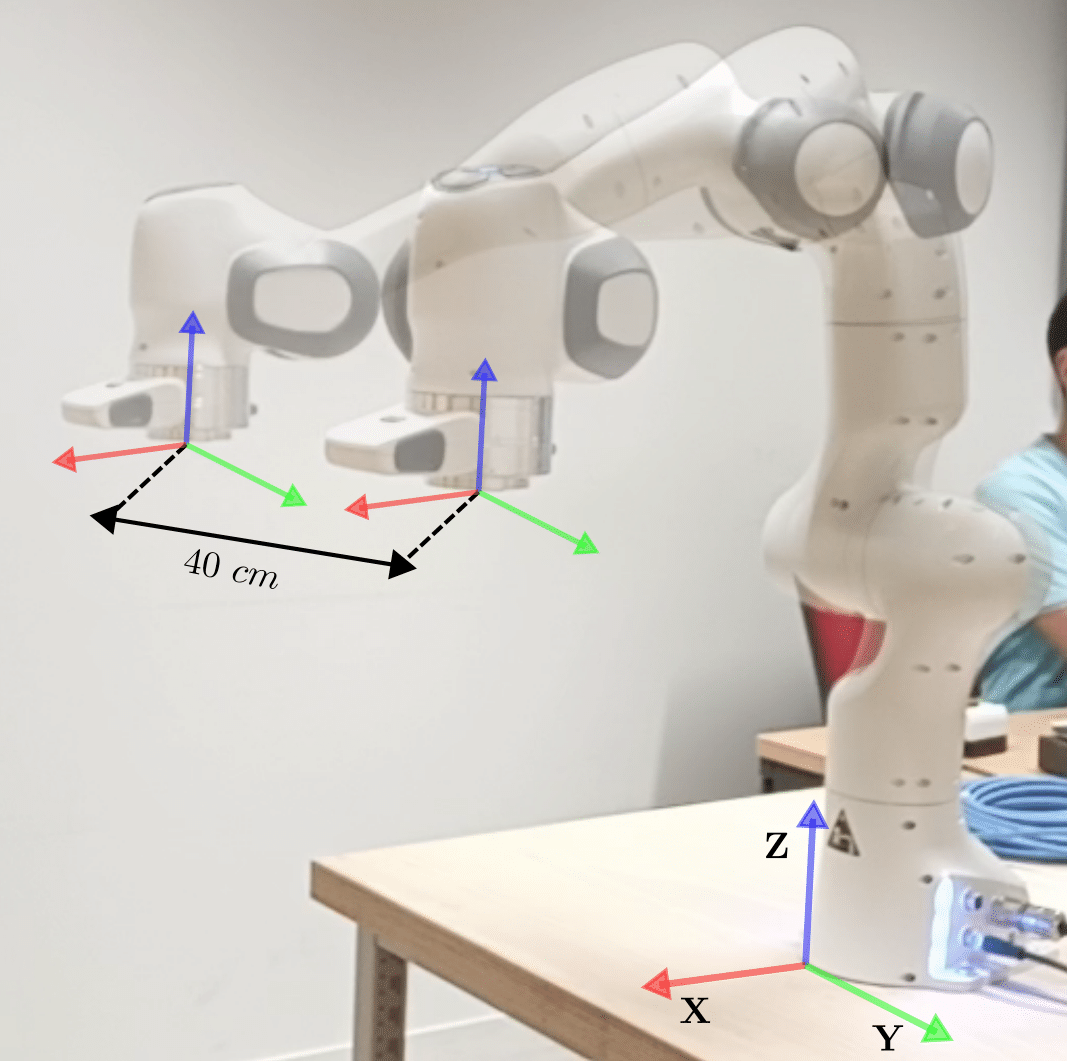
\includegraphics[width=0.45\columnwidth]{Panda_snap-cropped2-1.png}
	\includegraphics[width=0.45\columnwidth]{2Panda}
	\caption{Two superposed snapshots showing Panda end-effector converging to the two defined set-point pose targets.}
	\label{fig:panda_snap}
\end{figure}


\begin{figure}%[ht]
	\centering
	\subfloat[]{
		\includegraphics[width=0.455\columnwidth]{Panda_Fail.pdf}
		\label{subfig:pandaFail_Task}}
	\subfloat[]{
		\includegraphics[width=0.455\columnwidth]{Panda_Success.pdf}
		\label{subfig:pandaSuccess_Task}}
	\hfil
	\subfloat[]{
		\includegraphics[width=0.455\columnwidth]{jointAcceleration_fail.pdf}
		\label{subfig:pandaFail_u}}
	%	\hfil
	\subfloat[]{
		\includegraphics[width=0.455\columnwidth]{jointAcceleration_success.pdf}
		\label{subfig:pandaSucess_u}
	}
	\caption{Panda response for the ‘pick-and-place’ task under different feedback controls. End-effector Cartesian coordinates and $\jointCrtlIn$ evolution under: output feedback~\cref{eq:mu output feedback} \subref{subfig:pandaFail_Task}--\subref{subfig:pandaFail_u},  heterogeneous feedback~\cref{eq:heterogeneous feedback mu} \subref{subfig:pandaSuccess_Task}--\subref{subfig:pandaSucess_u}. The horizontal scales under \subref{subfig:pandaFail_Task} and \subref{subfig:pandaSuccess_Task} denote the stiffness gain $\taskStiffness$ within different time periods.} % \subref{subfig:pandaFail_Task}--\subref{subfig:pandaFail_u}  output feedback~\cref{eq:mu output feedback}. \subref{subfig:pandaSuccess_Task}--\subref{subfig:pandaSucess_u} End-effector Cartesian coordinates and $\jointCrtlIn$ evolution under heterogeneous feedback~\cref{eq:heterogeneous feedback mu}. The horizontal scales under \subref{subfig:pandaFail_Task} and \subref{subfig:pandaSuccess_Task} denote the stiffness gain within different time periods.}
\label{fig:pandaExperiment}
\end{figure}

%The same simulation scenario in \cref{subsubsec:control challenge for constraint} is conducted with RECBF constraint~\cref{eq:RECBF formulation}. Figure~\ref{fig:RECBF} shows the effect of tuning $\integralBfunc$ on the resulting dynamics. Robust safety is ensured despite the non-modeled joint-dynamics and external disturbance. 

\begin{figure}[ht]
	\centering
	\subfloat[]{
		\includegraphics[width=0.5\columnwidth]{Joint2VelocityTracking-Fail}
		\label{subfig:panda-velTracking-Fail}}
	%	\hfil
	\subfloat[]{
		\includegraphics[width=0.5\columnwidth]{Joint2VelocityTracking-Success}
		\label{subfig:panda-velTracking-Success}}
	\caption{Joint velocity tracking of the 2$^{\text{th}}$ joint.~\subref{subfig:panda-velTracking-Fail} Closed-loop system under output feedback~\cref{eq:mu output feedback} at stiffness $\taskStiffness=500$ leads to instability shown as fast oscillation of $\desConfDot$ tracked by $\actConfDot$. \subref{subfig:panda-velTracking-Success} Closed-loop system under heterogeneous feedback~\cref{eq:heterogeneous feedback mu} at stiffness $\taskStiffness=800$ where $\desConfDot$ is kept bounded even though it is not well tracked by $\actConfDot$, leading to a stable response.}
	\label{fig:panda-velTracking}
\end{figure}
\begin{figure}
	\centering
%	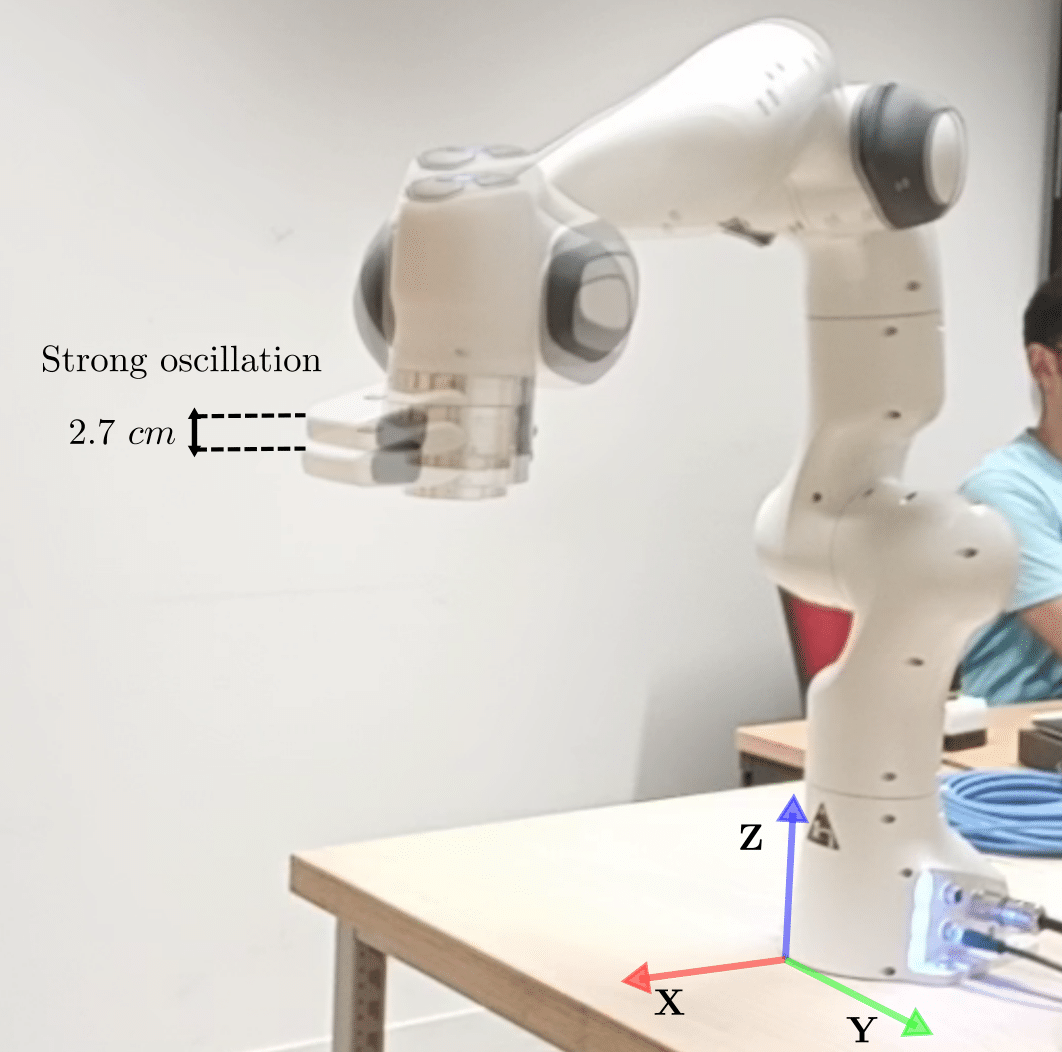
\includegraphics[width=0.5\columnwidth]{panda_vibration2-cropped2-1.png}
	\includegraphics[width=0.5\columnwidth]{panda_vibration2-cropped3}
	\caption{Strong oscillations (highlighted in yellow spot in \cref{fig:pandaExperiment}\subref{subfig:pandaFail_Task}) due to non-robustness of output feedback control~\cref{eq:mu output feedback}. The two superposed snapshots are taken with a time interval of $ T = 133$~ms.}
	\label{fig:panda_vib}
\end{figure}
\subsection{Sufficient Conditions for Lipschitz Continuity of Robust QP Solutions}\label{subsec-chap3:Robust QP Lipschitz continuity}
Since~\cref{eq:heterogeneous feedback mu} and~\cref{eq:RECBF formulation} are affine in $\UgenDesJointDyn$, the tasks and constraints can be combined by means of the following weight-prioritized QP efficiently solved online
%By replacing~\cref{eq:heterogeneous feedback mu} and~\cref{eq:RECBF formulation} in~\cref{eq:QP for combination}, the generalization to the weight-prioritized multi-objective robust QP control yields to 
\begin{subequations}\label{eq:robust QP for combination}
	\begin{align}
		\UgenDesJointDyn=\arg\min& \frac{1}{2}\UgenDesJointDyn^T\mathbf{H}(\genDesJointDyn)\UgenDesJointDyn + \bm{h}(\genDesJointDyn,\genActJointDyn)^T\UgenDesJointDyn\\
		\label{subeq:QP inequality constraint}\text{s.t: } &\mathbf{C}_{\mathrm{ineq}}(\genDesJointDyn)\UgenDesJointDyn\leq \bm{d}_{\mathrm{ineq}}(\genDesJointDyn,\genActJointDyn)\\
		\label{subeq:contact constraint}
		&\mathbf{C}_{\mathrm{eq}}(\genDesJointDyn)\UgenDesJointDyn= \bm{d}_{\mathrm{eq}}(\genDesJointDyn,\genActJointDyn)\\
		\label{subeq:G}\mathbf{H}(\genDesJointDyn) &= \sum_{i}\weight_{\fkini}{\desJacTaski}\tp\desJacTaski + \weight_0\selectMat\tp\selectMat\\
		\label{subeq:g}\bm{h}(\genDesJointDyn,\genActJointDyn) &=\sum_{i}\weight_{\fkini}{\desJacTaski}\tp (\desJacDotTaski\genDesConfDot + \taskGainsPsii\taskPsii  -  \fkinRefDDot^i(t))+ \weight_0\selectMat\tp \boldsymbol{\kappa}(\actJointDyn)\\
		\label{subeq:Cineq}\mathbf{C}_{\mathrm{ineq}}(\genDesJointDyn) &=-\desJacBfunc\\  
		\label{subeq:cineq}\bm{d}_{\mathrm{ineq}}(\genDesJointDyn,\genActJointDyn)&= \desJacBfuncDot\genDesConfDot + \constraintGainsPsi\bfuncPsi\\
		\label{subeq:Ceq}\mathbf{C}_{\mathrm{eq}}(\genDesJointDyn) &=\desJacContact\\  
		\label{subeq:ceq}\bm{d}_{\mathrm{eq}}(\genDesJointDyn,\genActJointDyn)&= \desJacContactDot\genDesConfDot %-\kappa\desJac^{\mathrm{c}}\genDesConfDot
	\end{align}
\end{subequations} with the superscript $(.)^i$ denotes the task $\fkini$. $\weight_{\fkin}$ is positive semi-definite weight and $\weight_0$ is any strictly positive infinitesimal weight~\cite[Lemma~2]{bouyarmane2018tac} of a secondary task that solves the remaining redundancy, with $\selectMat$\footnote{For a fixed-base robot, $\selectMat= \mathbf{I}_n$.} is the selection matrix and  $\boldsymbol{\kappa}(\actJointDyn)$ is a given joint-space feedback. It can be  a full configuration (posture) task~\cite{bouyarmane2011iros} or a velocity regulation task~\cite{basso2020ifac}. Inequality constraint~\eqref{subeq:QP inequality constraint} denotes the RECBF formulation ensuring robust stability of $\setCd$, whereas~\cref{subeq:contact constraint} stands for the no-slipping contacts at the feet as in~\cref{eq-chap1:contact constraint}  to have  feasible floating-base solutions $\FBCrtlIn$ where $\desJacContact$ is the contact Jacobian.

It is important to investigate the Lipschitz continuity of $\UgenDesJointDyn$ as it implies the existence and uniqueness of the closed-loop system solutions. Since~\cref{subeq:G} is symmetric positive-definite~\cite[Lemma~2]{bouyarmane2018tac} and~\cref{subeq:Ceq} is non-singular, and assuming that~\cref{subeq:G}--\cref{subeq:ceq} are Lipschitz continuous w.r.t $\genDesJointDyn$ and $\genActJointDyn$, then according to~\cite[Theorem~1]{morris2013cdc}\cite[Theorem~3]{ames2017tac}  $\UgenDesJointDyn$ is unique and Lipschitz continuous.  

Due to the subsequent conflicts that may arise between the different tasks, each task $\fkini$ is likely to be achieved partially according to the associated weight $\weighti$ and the possible active constraints\footnote{An inequality constraint is active if it is enforced as equality.} in QP~\eqref{eq:robust QP for combination}. This implicit relaxation is expressed as % The conflict between robust stabilization and robust safety is mediated by the implicit relaxation of~\cref{eq:heterogeneous feedback mu} w.r.t~\cref{eq:RECBF formulation}, and which can be expressed as 
\begin{equation}\label{eq:heterogeneous feedback relaxed}
	\taskCrtlIni = -\taskGainsPsii\taskPsii+ \bm{\delta}^{\fkini}(t)
\end{equation} 
with $\bm{\delta}^{\fkini}(t)\in\mathbb{R}^{m}$ assumed to be bounded $\norm{\bm{\delta}^{\fkini}(t)}\leq\delta^{\fkini}_{\max}, \forall t \geq0$. 
%In addition, it encodes the conflict that may occur between several tasks in the case of multi-objective control. All in all, if a task is relaxed, it is likely to be achieved partially.
% Consequently, the implication of relaxation in terms of stability needs to be investigated.  %By considering $\delta(t)$ as a disturbance input, it happens that the relaxation effect can be suitably studied using the ISS notion~\cite{sontag2008springer}.  
\cref{prop:relaxed heterogeneous feedback} generalizes \cref{thm:heterogeneous feedback} to  the case of multi-objective control.%shows that~\cref{eq:heterogeneous feedback relaxed} leads to uniform ultimate boundedness of $\actTaskOut $. 
\begin{proposition}\label{prop:relaxed heterogeneous feedback}
	Consider~\cref{eq:heterogeneous feedback relaxed}  such that \cref{thm:heterogeneous feedback} conditions hold. Then, there exists $\taskIntegralDampingi\in\mathbb{R}^{m\times m}$ positive-definite such that $\desTaskOuti$ is practically robustly stable. %is uniformly ultimately bounded.
\end{proposition}
\begin{custumProof}{Proof}
	See \cref{proof:prop3}.
\end{custumProof}
Note that by the virtue of \cref{prop:relaxed heterogeneous feedback}, \cref{thm:RECBF} and \cref{prop 1}, $\genDesJointDyn$ is stable (bounded) after double integration of $\UgenDesJointDyn$ solution of QP~\eqref{eq:robust QP for combination}.
%{\color{red}Note that by the virtue of Propositions~\ref{prop 1},~\ref{prop:relaxed heterogeneous feedback} and~\ref{thm:RECBF}, $\genDesJointDyn$ is stable after double integration of $\UgenDesJointDyn$ solution of~\cref{eq:robust QP for combination}.}

\begin{remark}\label{rem:decision variables}
	In QP~\eqref{eq:robust QP for combination}, only one RECBF constraint is considered. In the more general case, the QP constraints set encompasses:  (i) several RECBFs (joint constraints, collision avoidance, CoM equilibrium region, etc.), (ii) EoM~\eqref{eq-chap0:equation of motion} for dynamic consistency, and (iii) explicit bounds on $\jointCrtlIn$. Therefore, we highlight two important aspects: First, \cref{thm:RECBF} assumes that ${\cal U}=\mathbb{R}^{6+n}$ which may not hold. Second, since all the constraints have the same  priority level, the QP will fail if these constraints are in conflict~\cite{decre2009icra,rubrecht2010iros,delprete2018ral}. An approach to solve this issue is proposed in \cref{chap:mpc ref gov}.
\end{remark}
\begin{remark}
		In QP~\eqref{eq:robust QP for combination}, only the desired acceleration $\genDesConfDDot$ is considered as a decision variable to show explicitly how the QP is constructed to combine robust task stability (\cref{eq:heterogeneous feedback mu}) and set robust stability (\cref{eq:RECBF formulation}).  Having $\desForce$ as an additional decision variable in QP~\eqref{eq:robust QP for combination} does not call for a particular consideration since we are so far interested in terminal points governed by free motion tasks. From in implementation standpoint, $\desForce$ are formulated as in~\eqref{eq-chap0:force constraint} to remain inside the friction cone.
\end{remark}


\subsection{Comparison with State-of-the-Art}\label{sec-chap2:sota chap2}
The instability issue of the closed-loop task-space QP controller combined with a kinematic-controlled robot has been unnoticed in some control implementations that operate in feedforward (\cref{fig:QP scheme for kinematic-control robots}\subref{subfig:feedforward QP})~\cite{bouyarmane2018tac,zanchettin2017elsevier,polverini2017iros_a,shi2022machines}. This leads to a decoupled control (similar to~\cite{feng2015journalOfFieldRobotics}), delegating the control accuracy to the joint-controllers. In such cases, frequent initializations of the controller are needed to lower the discrepancy between real and control-model states due to non-modeled flexibilities or external disturbance. 


Most of the works reporting instability are those using torque-controlled robots with numerically-implemented joint-controllers (\cref{fig:leaky integrator QP}), see e.g.,~\cite{feng2015journalOfFieldRobotics,johnson2015journalOfFieldRobotics,dedonato2017frontiers,koolen2016ijhr}. Interestingly, it has been noted in~\cite{feng2015journalOfFieldRobotics} that the oscillations and undesired behaviors are related to the double integration of the QP output $\desConfDDot$. However, no further investigation was made to elucidate the cause. 
Instead, only workaround solutions have been proposed to bypass this issue.

~\cite{hopkins2015icra} implemented a joint-velocity feedback on $\genActConfDDot$ computed by QP (denoted as \emph{leaky-integrator})
\begin{equation}\label{eq:leaky-integrator}
	\genActConfDDot^{\rm LI} = \genActConfDDot - \alpha \left(\genActConfDot^{\rm LI} - \genActConfDot\right) , \ \alpha>0.   
\end{equation}
 %similar to the joint-space integral feedback discussed in~\cref{chap:instable qp}. 
 The authors reported qualitatively that the leaky-integrator enhances the overall stability. Nevertheless, they did not provide clear insights on how the leaky-integrator gain $\alpha$ improves the stability nor how to tune it. Our work has been inspired by the leaky-integrator scheme~\eqref{eq:leaky-integrator}. However, it differs in two points: (i) the integral feedback is formulated at the task-space\footnote{The leaky-integrator \cref{eq:leaky-integrator} is recovered in the joint-space integral feedback \cref{eq:heterogeneous feedback 1DoF closedLoop} discussed in~\cref{chap:instable qp} when $\genActConfDDot$ is formulated as a PD feedback.}; and (ii) the integral term is added directly to the task feedback in QP cost-function and not post QP-computation which does not affect the optimality of QP solution conversely to~\cref{eq:leaky-integrator}. 
 
 To mitigate this issue, other approaches accounted for the joint-feedback in QP.~\cite{cisneros2018iros} accounted for the velocity feedback in the dynamics and non-slipping constraint to ensure the feasibility of desired acceleration. However, the authors also considered the velocity feedback term on the underactuated part of the equation of motion (in the case of a humanoid robot), which significantly alters the dynamics and raises questions about the meaning of such \emph{virtual} dynamics.
 
 Conversely,~\cite{feng2014humanoids,feng2015journalOfFieldRobotics} changed the QP architecture drastically by proposing a mixture between ID-QP and IK-QP where the latter computes the desired joint position and velocity (required by the joint-controllers) based on the feedforward scheme~\cref{fig:QP scheme for kinematic-control robots}\subref{subfig:feedforward QP}. However, the approach leaks formal stability proofs where only experimental evidence has been provided. 
%These palliative methods can be sorted into two categories: (i) \emph{low-level approaches} that act at the joint-level to prevent $\desConfDDot$ double integration from diverging typically by implementing a leaky integrator~\cite{hopkins2015icra} similar to the joint-space integral feedback discussed in~\cref{chap:instable qp}; and (ii) \emph{high-level approaches}  where the QP formulation is substantially modified at the expense of a complex control-architecture~\cite{feng2014humanoids,feng2015journalOfFieldRobotics}, or by accounting for the joint feedback terms in the QP to adapt their gains~\cite{lee2022frontiersRobS} or for constraints feasibility concerns~\cite{cisneros2018iros}. 
%The former do not provide a clear insights of how the leaky-integrator gain improves the stability nor how to tune it, whereas the latter yield to a complex QP formulation and leaks of formal stability proofs where only experimental evidences have been provided. 

Other approaches resorted to lowering the task gains to mitigate the instability~\cite{koolen2016ijhr,johnson2015journalOfFieldRobotics}. 

More related to kinematic constraint formulation, it has been shown in \cite{singletary2022csl,molnar2022ral} that choosing high CBF gain leads to oscillations at the constraint boundary depending on the joint-dynamics. An energy-based CBF has been proposed to ensure conservative stability of the set $\setC$. However, the joint-dynamics model and parameters must be known. 
%Similar observation is made in~\cite{djeha2020ral,singletary2022csl} concerning the gains of the safety-constraint formulation. 

%Moreover,  the robots used in the above cited works rely also on joint-controllers in addition to a feedforward torque term (\cref{fig:leaky integrator QP}). The only difference with robots in \cref{fig:position controller} is the joint-controllers are numerically-implemented, whereas  they are hardware-implemented  for kinematic-controlled robots.  
 
%Several research works reported instability phenomena of relative severity (e.g., strong sustained oscillations), see e.g.,~\cite{feng2015journalOfFieldRobotics,johnson2015journalOfFieldRobotics,dedonato2017frontiers,koolen2016ijhr}. Interestingly, the common factor in each reported shortcoming is that the joint torque control relies on joint-position and/or velocity feedback terms in addition to $\desTau$ (\cref{fig:leaky integrator QP}). In~\cite{feng2015journalOfFieldRobotics}, it has been noted that the oscillations and undesired behaviors are related to the double integration of the QP output $\desConfDDot$. However, no further investigation was made to elucidate the cause.
 
%Several research works have reported similar instability phenomena of relative severity (e.g., strong sustained oscillations), see e.g.,~\cite{feng2015journalOfFieldRobotics,johnson2015journalOfFieldRobotics,dedonato2017frontiers,koolen2016ijhr}. Interestingly, it has been noted in~\cite{feng2015journalOfFieldRobotics} that the oscillations and undesired behaviors are related to the double integration of the QP output $\desConfDDot$. However, no further investigation was made to elucidate the cause. Instead, only workaround solutions have been proposed to bypass this issue. 
%Moreover,  the robots used in the above cited works rely also on joint-controllers in addition to a feedforward torque term (\cref{fig:leaky integrator QP}). The only difference with robots in \cref{fig:position controller} is the joint-controllers are numerically-implemented, whereas  they are hardware-implemented  for kinematic-controlled robots.  
 
%Workaround solutions have been proposed to mitigate this issue. These palliative methods can be sorted into two categories: (i) \emph{low-level approaches} that act at the joint-level to prevent $\desConfDDot$ double integration from diverging; typically by implementing a leaky integrator~\cite{hopkins2015icra}; and (ii) \emph{high-level approaches}  where the QP formulation is substantially modified at the expense of a complex control-architecture~\cite{feng2014humanoids,feng2015journalOfFieldRobotics}, or by accounting for the joint feedback terms in the QP to adapt their gains~\cite{lee2022frontiersRobS} or for constraints feasibility concerns~\cite{cisneros2018iros}. Other approaches reported that lowering the task gains helps mitigating the instability~\cite{koolen2016ijhr,johnson2015journalOfFieldRobotics} which highlights the fact that task gains are also an interfering factor. Similar observation is made in~\cite{djeha2020ral,singletary2022csl} concerning the gains of the safety-constraint formulation. 

%The closed-loop task-space QP controller combined with a joint low-level kinematic-controlled robot,~\cref{fig:QP scheme for kinematic-control robots}\subref{subfig:feedback QP}, is also prone to previously described instability shortcomings.  
%The latter have been unnoticed in some control implementations that operate in feedforward (\cref{fig:QP scheme for kinematic-control robots}\subref{subfig:feedforward QP}). This leads to a decoupled control (similar to~\cite{feng2015journalOfFieldRobotics}), delegating the control accuracy to the joint controllers~\cite{bouyarmane2018tac,zanchettin2017elsevier,polverini2017iros_a}. In such cases, frequent initializations of the controller are needed to lower the discrepancy between real and control-model states due to non-modeled flexibilities or external disturbance. 

%\emph{Remark~\showmycounter{rem2}:}  
\section{Experimental Results and Discussion}\label{sec-chap3:Experiments}
To assess our robust QP controller and demonstrate its applicability to different use-cases, experiments are conducted with two different robots: a fixed-base 7-DoF robotic arm Panda from Franka Emika, and a (floating-base) 34-DoF humanoid robot HRP-4 from Kawada Robotics. The latter is controlled in position at a frequency of $200$~Hz. In contrast, the former can be controlled either in position or velocity modes at a control frequency of $1$~kHz. 

Both robots are controlled using the open source code implementation of the QP controller \mcrtc. % that includes user task specification interface, debugging, data recording... for simulation as well as for real-time control. 
Based on the embedded sensors data (encoders, IMU, Force/Torque (F/T) sensors, etc.), \mcrtc~builds at each control-cycle the QP problem, based on user-defined tasks and constraints, and solves it. The QP decision variables are $\UgenDesJointDyn$ and the contact forces $\desForce$. 
\begin{figure}
	\centering
	\includegraphics[width=0.65\columnwidth]{COM_withAxis_shrinked_arrows}
	\caption{Top-view of the humanoid robot HRP-4. The equilibrium polygon is shown in red vertices, the CoM in a yellow dot and the vertices normal vector in orange. The polygon is a rectangle in ${XY}$ plane such that ${X}_{\max} = 5$~cm, ${X}_{\min} = -2$~cm, ${Y}_{\max} = 5$~cm, ${Y}_{\min} = -5$~cm.}
	\label{fig:CoM polgon}
\end{figure}
%Having $\desForce$ as an additional decision variable in QP~\eqref{eq:robust QP for combination} does not call for a particular consideration. So far, we are interested in terminal points governed by free motion tasks. 
Each contact force between HRP-4 feet and the floor are yet enforced by \cref{eq-chap0:force constraint} to remain within their linearized friction cone and prevent slippage. %, which is expressed as 
%\begin{equation}\label{eq:contact forces}
%	f = \sum_{j=1}^{n_c} \beta_j\rho_j, \ \beta_j \geq0 
%\end{equation} where $\rho_j\in\mathbb{R}^3$ is the $j^{\text{th}}$ vertex of the linearized friction cone. %~\cite{bouyarmane2011iros}. 
Then, $\UgenDesJointDyn$ and $\desForce$ are coupled through the dynamics constraint~\eqref{eq-chap0:tau bounds} to enforce QP to generate feasible and dynamically-consistent solutions of the floating-base $\FBCrtlIn$.
%\begin{equation}\label{eq:dynamics constraint}
%	S_{\tau} \tau_{\min}\leq M(\genActConf)\UgenDesJointDyn + N(\genActConf,\genActConfDot) - \bar{\actJac}^{\mathrm{c}^T}f \leq S_{\tau} \tau_{\max}
%\end{equation} where $M(\genActConf)\!\in\!\mathbb{R}^{(6+n)\times(6+n)}$ is the inertia matrix, $N(\genActConf,\genActConfDot)\!\in\!\mathbb{R}^{6+n}$ accounts for Coriolis, centrifugal and gravity effects, $\bar{\actJac}\!\in\!\mathbb{R}^{3\times(6+n)}$ is the linear part of the contact Jacobian, $S_{\tau}\!\in\!\mathbb{R}^{(6+n)\times n}$ is the actuation selection matrix, and $\tau_{\min},\tau_{\max}\!\in\!\mathbb{R}^n$ are the joint torque bounds. 
%\cref{subeq:contact constraint},~\ref{eq:contact forces} and~\cref{eq:dynamics constraint} enforce QP to generate feasible and dynamically-consistent solutions of the floating-base $\FBCrtlIn$.
\begin{figure}
	\centering
	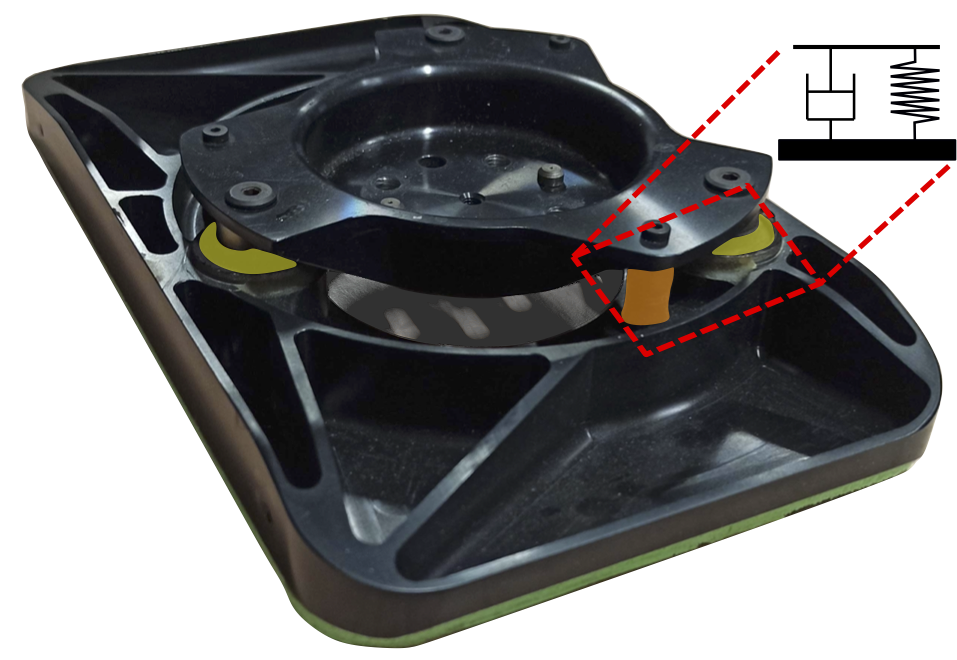
\includegraphics[width=.5\columnwidth]{feet flexibilities2-model3.png}%{HRP-soles-highlight}
	\caption{Rubber bushes (yellow) and dampers (orange) under HRP-4 ankles (highlighted in yellow) that induce non-modeled flexibilities.}
	\label{fig:hrp soles}
\end{figure}

\begin{figure}
	\centering
	\subfloat[]{
		\includegraphics[width=0.5\columnwidth]{ECBF OL COM.pdf}
		\label{subfig:com_OL}
	}%\hfil
	\subfloat[]{
		\includegraphics[width=0.5\columnwidth]{feedback CL-time.pdf}
		\label{subfig:com_CL}
	}\hfil
	\subfloat[]{
		\includegraphics[width=0.5\columnwidth]{robust RECBF COM-TimeSlot.pdf}
		\label{subfig:com_Robust}}
	%		}\hfil
%		\subfloat[]{
	%			\includegraphics[width=\columnwidth]{push COM.pdf}
	%			\label{subfig:com push}}
\caption{Time Evolution of $\actCoM$, $\desCoM$ and their respective velocities coordinates along ${X}$ and ${Y}$ axes.~\subref{subfig:com_OL} Experiment~\ref{exp-cha3:feedforward ECBF}.~\subref{subfig:com_CL} Experiment~\ref{exp-cha3:feedback ECBF}.~\subref{subfig:com_Robust} Experiment~\ref{exp-cha3:RECBF}. The gray time slot is zoomed-in in \cref{fig:com_Robust Zoom}.}
\label{fig:com}
\end{figure}
\begin{figure}
	\centering
	\includegraphics[width=0.6\columnwidth]{Zoom Robust RECBF.pdf}
	\caption{Zoom-in of the gray time slot in \cref{fig:com}\subref{subfig:com_Robust}. The bold dashed line denotes the moment when the RECBF constraint relative to $\mathbf{X}_{\max}$ boundary is inserted in QP~\cref{eq:robust QP for combination}.}
	\label{fig:com_Robust Zoom}
\end{figure}
\begin{figure}
	\centering
	\includegraphics[width=0.6\columnwidth]{ECBF-CL-DesiredForces}
	\caption{Desired contact forces computed by QP during failed Experiment~\cref{exp-cha3:feedback ECBF}. The required desired forces for decelerate the whole-body are excessively high and cannot fulfill the frictional constraint~\eqref{eq-chap0:force constraint}.}
	\label{fig:desired Forces}
\end{figure}
\begin{figure}
	\centering
	\includegraphics[width=0.6\columnwidth]{torque Cy}
	\caption{Torque measurements w.r.t ${Y}$ axis showing the feet tip-over at Experiment~\cref{exp-cha3:feedback ECBF}. Given the placement of the F/T sensors in \cref{fig:hrp soles}, a torque of $-22$~Nm denotes a force of approximately $220$~N along ${Z}$ axis at the backward edge of each foot which is the amount of force sensed at each foot when the robot is standing.}
	\label{fig:tip over torque}
\end{figure}
As it is shown in~\cref{eq:double integrator} and~\cref{fig:whole control scheme}, $\UgenDesJointDyn$ is integrated twice to obtain $\genDesJointDyn$, then the joint commands $\desJointDyn$ are sent to the actuated joint-controllers. The joint-velocity is estimated using numerical derivation for HRP-4, whereas it is delivered by the Franka Control Interface (FCI) for Panda\footnote{The FCI joint-velocity estimation is a low-pass filtered finite-difference.}. The floating-base state $\actFBDyn$ in~\cref{eq:gen joint dyn def} of HRP-4 is estimated by a built-in kinematic-inertial observer based on an extended Kalman filter. 
%The control is performed using a laptop Dell Precision~5540 with Intel Xeon(R)~E-2276M processor (CPU $12 \times  2.80$~GHz) and $31$~GB of RAM running under Linux Ubuntu~18.04.5 LTS.

\begin{figure}
\centering
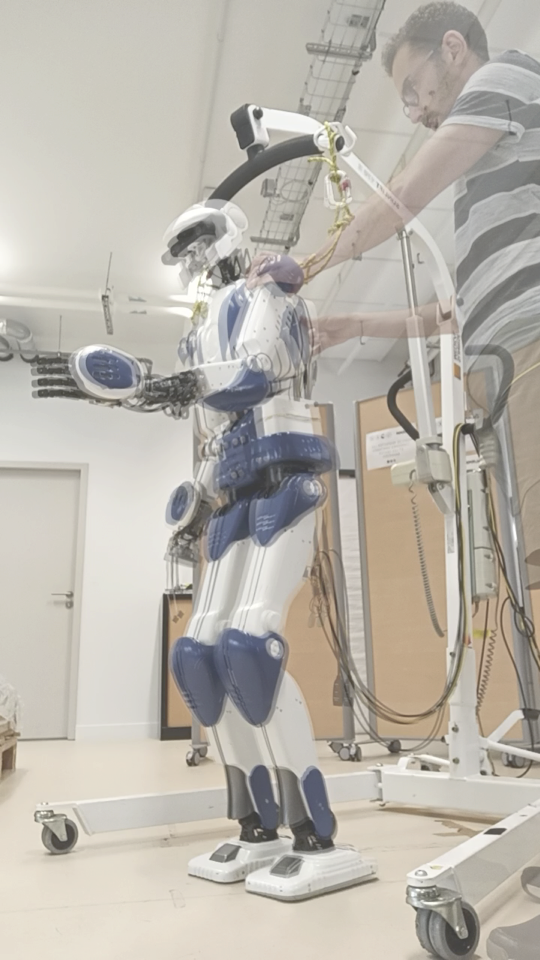
\includegraphics[width=0.4\columnwidth]{snap1-1.png}
%\includegraphics[width=0.32\columnwidth]{snap2}
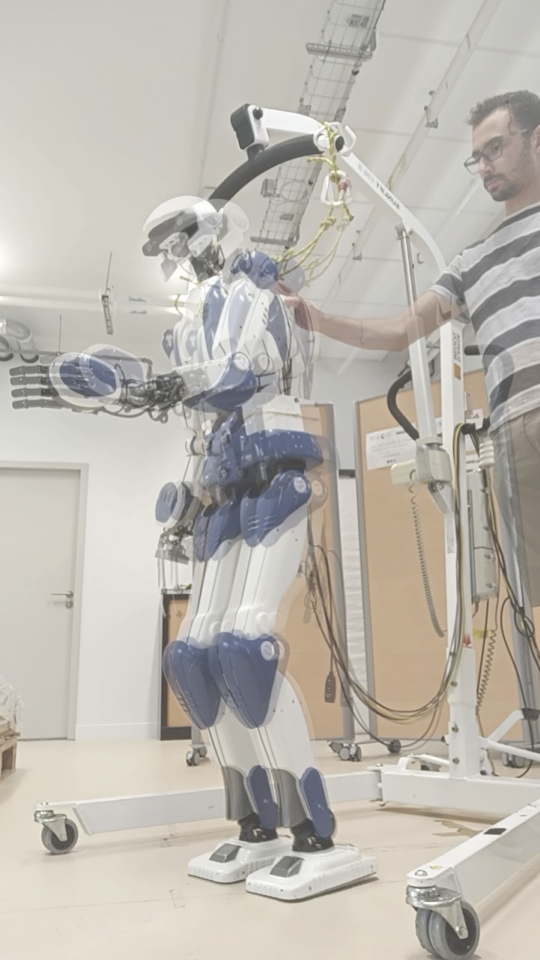
\includegraphics[width=0.4\columnwidth]{snap3-1.png} \\
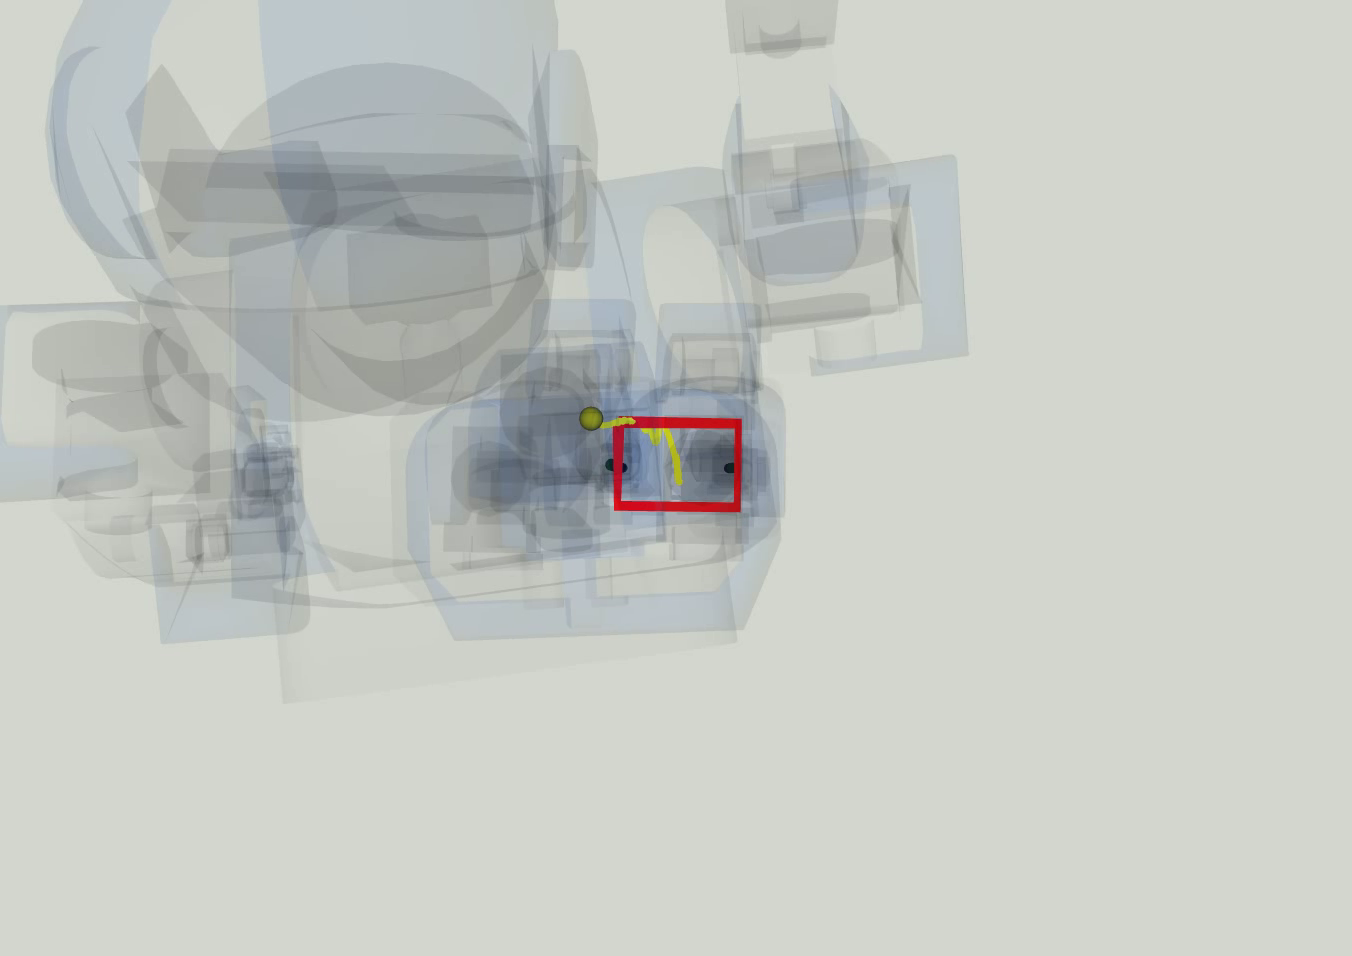
\includegraphics[width=0.4\columnwidth]{voko1}
%\includegraphics[width=0.32\columnwidth]{snap2}
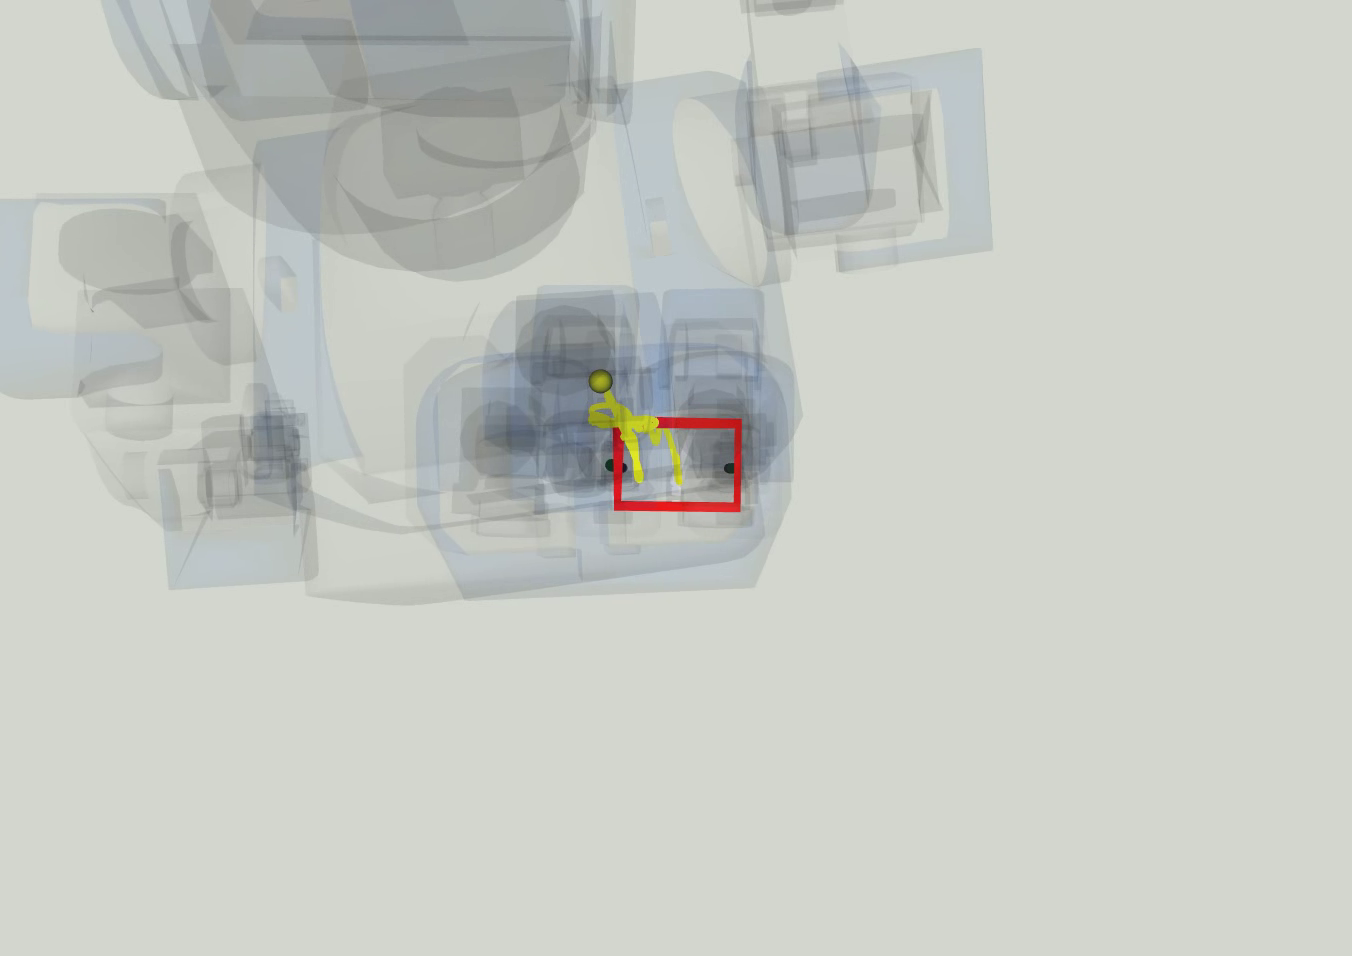
\includegraphics[width=0.4\columnwidth]{voko3} \\
\caption{Superposed snapshots of robust against pushing (experiment 4) along ${X}$ (right-top) and ${Y}$ (left-top) directions, with the corresponding top-view perspectives (bottom).}
\label{fig:com push snapshots}
\end{figure}
%\begin{figure}
%\centering
%\includegraphics[width=0.8\columnwidth]{RECBF push-TimeSlots.pdf}
%\caption{Robustness of RECBF~\cref{eq:RECBF formulation} against external pushes. The blue time slot denotes a persistent external push (\cref{fig:zoom com push}\subref{subfig:com persistent push}), and the green one denotes a brief external push (\cref{fig:zoom com push}\subref{subfig:com brief push}).}
%\label{fig:com push}
%\end{figure}
%	\begin{figure}
%		\centering
%		\includegraphics[width=\columnwidth]{RECBF push COM-Zoom.pdf}
%		\caption{Zoom-in the blue time slot in~\cref{fig:com push} showing the response against a persistent external push.}
%		\label{fig:com persistent push}
%	\end{figure}
%	\begin{figure}
%		\centering
%		\includegraphics[width=\columnwidth]{RECBF push COM-Brief-Zoom.pdf}
%		\caption{Zoom-in the green time slot in~\cref{fig:com push} showing the response against a persistent brief push.}
%		\label{fig:com brief push}
%	\end{figure}
\begin{figure}
\centering
\subfloat[]{
\includegraphics[width=0.5\columnwidth]{RECBF push-TimeSlots.pdf}
\label{subfig:com push}
}
%\hfil
\subfloat[]{
\includegraphics[width=0.5\columnwidth]{RECBF push COM-Zoom.pdf}
\label{subfig:com persistent push}
}
\hfil
\subfloat[]{
\includegraphics[width=0.5\columnwidth]{RECBF push COM-Brief-Zoom.pdf}
\label{subfig:com brief push}
}
\caption{ Robustness of RECBF~\cref{eq:RECBF formulation} against external pushes. \subref{subfig:com persistent push} Zoom-in of the blue time-slot in~\subref{subfig:com push} showing the response against a persistent external push. \subref{subfig:com brief push} Zoom-in of the green time slot in~\subref{subfig:com push} showing the response against a brief push.}
\label{fig:com push}
\end{figure}

% \begin{figure}
%	\centering
%	\includegraphics[width=\columnwidth]{IAM}
%	\caption{Illustrative example of robots integration in industrial process (\url{http://www.i-am-project.eu/index.php}).}
%	\label{fig:IAM}
%\end{figure}
\subsection{Task Robust Stability}\label{subsec-chap3:experiment_robust stability} 
%	\phantom{in applications where settle time and accuracy are required.}
The task gains correlate to accuracy (performing motions with high precision) and execution speed (controlling the overall task time). In this context, the Panda end-effector is controlled to perform a pick-and-place-like motion. Two target set-points (position and orientation) are defined (to which the end-effector converges back and forth). To have simple plots, only the target coordinate along the $Y$-axis varies with an amplitude of $\pm20$~cm (\cref{fig:panda_snap}). In this experiment, $\desConfDot$ is the desired joint commands for the joint controllers (velocity mode).

QP~\cref{eq:robust QP for combination} is formulated\footnote{Since Panda is a fixed-base robot, the notations in \cref{rem:fixed-base robot case} are followed in \cref{subsec-chap3:experiment_robust stability}.} such that the constraint set contains the kinematic constraints (joint-position and velocity constraints~\cite{djeha2020ral}); whereas, for comparison purpose, the task is formulated using: (i) output feedback~\cref{eq:mu output feedback}, (ii) heterogeneous feedback~\cref{eq:heterogeneous feedback mu}. 
The task gains are set as $\taskDamping=2\sqrt{\taskStiffness}$ and $\taskIntegralDamping= \epsilon \taskDamping$ with $\varepsilon=0$ for~\cref{eq:mu output feedback} and $\varepsilon=1$ for~\cref{eq:heterogeneous feedback mu}. $\taskStiffness$ is initially set to $400$,  then it is increased overtime by increments of $50$ ($\taskDamping$ and $\taskIntegralDamping$ are updated accordingly). 

The experiment results are shown in~\cref{fig:pandaExperiment}. For $\taskStiffness\leq 450$, both feedback controls~\eqref{eq:mu output feedback} and~\eqref{eq:heterogeneous feedback mu} lead to a stable convergence to the targets. However for  $\taskStiffness=500$, the closed-loop system with output feedback~\eqref{eq:mu output feedback} becomes instable (\cref{fig:pandaExperiment}\subref{subfig:pandaFail_Task}) where strong oscillation and discontinuous motion appear at the end-effector mostly visible along the $Z$-axis (\cref{fig:panda_vib}). This jerky motion can be very dangerous for the robot (it drastically accelerates  the wear of actuators and robot's structure) as well as the surrounding people or objects in the robot neighborhood. Conversely, heterogeneous feedback~\eqref{eq:heterogeneous feedback mu} allows to reach robustly the targets while $\taskStiffness$ keeps increasing up to $850$ (\cref{fig:pandaExperiment}\subref{subfig:pandaSuccess_Task}). 

Increasing the task gains results in high values of desired joint acceleration $\jointCrtlIn$ (\cref{fig:pandaExperiment}\subref{subfig:pandaFail_u}--\subref{subfig:pandaSucess_u}) which generates desired joint commands $\desConfDot$ with  fast variations that cannot be well tracked by the joint controllers (\cref{fig:panda-velTracking}\subref{subfig:panda-velTracking-Fail}--\subref{subfig:panda-velTracking-Success}) due to the different rate limitations (acceleration, jerk) and the limited bandwidth. This leads to increase the joint tracking error $\jointTrackErr$ in~\cref{eq:joint tracking error}, and correspondingly its task-space mapping $\taskTrackErr$ in~\cref{eq:DL act task}. 
%{\color{red}Consequently, if the perturbation term $K\taskTrackErr$ %in~\cref{eq:des task dyn around eq} 
%is not sufficiently bounded then the closed-loop system under output feedback~\cref{eq:mapping mu to u} becomes instable.} 
In particular, adding the task-space integral term in~\cref{eq:heterogeneous feedback mu} allows to withstand the perturbation by the gain $\taskIntegralDamping$ as shown in~\cref{eq:cdt on norm - Lv} enforcing $\desTaskOut $ to remain bounded which leads to the boundedness of $\desJointDyn $ (by the virtue of \cref{prop 1}). 

In~\cref{fig:pandaExperiment}\subref{subfig:pandaSuccess_Task}--\subref{subfig:pandaSucess_u}, we decided to stop at stiffness $\taskStiffness=850$ as, due to hardware limits, further increasing the task gains has no effect on the convergence performance (\cref{fig:panda-velTracking}\subref{subfig:panda-velTracking-Success}). Although the joint controllers reached their maximum tracking performances, our approach enables a stable motion even though the task gains keep increasing and imposing a desired dynamics that the robot cannot achieve. Hence, ensuring the closed-loop stability property is crucial, whatever the task gains and whatever the joint-dynamics.% Yet, this stability guaranty goes at the expanse of a conservative tuning of $\taskIntegralDamping$.  	

\subsection{Set Robust Stability}\label{subsec-chap3:expreiment_robust safety}%{Robust Safety}

As an example of a critical safety feature in humanoids is the dynamic balance (equilibrium) that is given a higher priority over the manipulation tasks. This is achieved by enforcing the CoM to remain inside a computed equilibrium region, e.g.,~\cite{audren2018tro,samadi2021ral}. 

In this experiment, a conservative CoM equilibrium polygon is defined for the humanoid robot HRP-4 (\cref{fig:CoM polgon}). A sequence of Cartesian targets is defined for the right hand to be reached. These targets are intended to bring the CoM to reach the polygon boundaries. Rubber bushes and dampers are present under the robot's ankles to absorb the impact at the feet while walking (\cref{fig:hrp soles}). This shock-absorbing mechanism creates uncontrolled flexibilities between the ankle and the feet, resulting in perturbations affecting the CoM and the estimations of the floating-base state. Moreover, the joints' steady-state tracking errors and the floating-base IMU noise affect the CoM estimation (denoted $\actCoM\in\mathbb{R}^3$). 

The robot CoM is constrained to remain within the equilibrium polygon by defining inequality constraints on the distance between $\actCoM$ and the polygon features.
Hence, the barrier functions $\bfunc^i$ and $\desBfunc^i$ corresponding to each equilibrium polygon feature $i$ are computed as 

\begin{align}
\label{eq:bfunc EXP}\bfunc^i & = \bm{n}^{i\tp}\actCoM + \Delta^i,\\
\label{eq:des bunc EXP}\desBfunc^i & = \bm{n}^{i\tp}\desCoM + \Delta^i,
\end{align} 
where $\bm{n}^{i}\in\mathbb{R}^3$ is the $i^{\text{th}}$ feature's normal vector and $\Delta^i\in\mathbb{R}$ is the distance at which the feature is placed w.r.t the origin. From~\cref{eq:bfunc EXP}--\cref{eq:des bunc EXP}, 	the sets $\setC^i$ and $\setC_d^i$ are defined as in~\cref{eq:act C}--\cref{eq:int act C} and~\cref{eq:des C}--\cref{eq:int des C}, respectively. QP~\eqref{eq:robust QP for combination} is formulated to steer the right hand to its targets. If $\bfunc^i\leq 4$~cm then the RECBF constraint~\cref{eq:RECBF formulation} is inserted into the constraint set of~\cref{eq:robust QP for combination}. Finally, contact forces constraint~\cref{eq-chap0:force constraint} is considered to have feasible and dynamically-consistent floating-base solutions $\FBCrtlIn$. Dynamic-consistency refers to the fact that the CoM deceleration generated by the RECBF relies (dynamically speaking) on the contact forces. 
In this experiment, $\desConf$ is the desired joint commands  for the joint controllers.

For comparison purpose, three identical experimental scenarios have been conducted using the different closed-loop QP control schemes shown in \cref{fig:QP scheme for kinematic-control robots}:

 \begin{experiment}{Experiment}\label{exp-cha3:feedforward ECBF}
	 ECBF constraint~\eqref{eq:ECBF constraint} following feedforward QP closed-loop control scheme (\cref{fig:QP scheme for kinematic-control robots}\subref{subfig:feedforward QP});
\end{experiment}
\begin{experiment}{Experiment}\label{exp-cha3:feedback ECBF}
	 ECBF constraint~\eqref{eq:ECBF constraint} following feedback QP closed-loop control scheme (\cref{fig:QP scheme for kinematic-control robots}\subref{subfig:feedback QP});
\end{experiment} 
\begin{experiment}{Experiment}\label{exp-cha3:RECBF}
	RECBF constraint~\cref{eq:RECBF formulation} following the proposed QP closed-loop control scheme (\cref{fig:whole control scheme}).
\end{experiment}



The results are shown in \cref{fig:com}. In the three experiments, the stiffness $\constraintStiffness$ is computed as shown in~\cite{djeha2020ral} (\cref{thm:RECBF}). For Experiments~\cref{exp-cha3:feedforward ECBF}--\cref{exp-cha3:feedback ECBF}, $\constraintDamping = 2.4\sqrt{\constraintStiffness}$. In Experiment~\cref{exp-cha3:feedforward ECBF} (\cref{fig:com}\subref{subfig:com_OL}), the robot state $\genActJointDyn$ is not fed-back to QP.  
We can see that $\desCoM$ is within the limits and the set $\setCd$~\eqref{eq:des C}--\eqref{eq:int des C} is rendered forward invariant. However, since the robot is not taken into account in the closed-loop system, forward invariance is not ensured for the set $\setC$~\cref{eq:act C}--\cref{eq:int act C}. The mismatch between $\desCoM$ and $\actCoM$  leads the latter to overshoot the  $X_{\max}$ limit with an amount of $2$~cm, then to completely drifts away from the equilibrium region  at $t=50$~s leading the robot to lose balance.

In Experiment~\cref{exp-cha3:feedback ECBF} (\cref{fig:com}\subref{subfig:com_CL}), the robot state is considered in closed-loop, but the ECBF formulation leads to instability. The bold dashed line shows the moment when ECBF constraint relative to ${X}_{\max}$ boundary is inserted. Instantaneously, $\desCoM$ velocity along ${X}$-axis starts to decrease (brown dash-dotted line). Nevertheless, $\actCoM$ velocity does not decrease immediately, causing $\actCoM$ to keep moving toward ${X}_{\max}$ boundary. This lag is due to the flexibility. 

In fact, the QP controller relies mainly on the ankles joints to move the CoM since the ECBF-produced deceleration is mapped mainly to the ankles joints through~\cref{eq:mapping Bfunc mu to u} because a little motion at the ankles leads to a larger motion of the robot whole-body. However, the flexibilities act like underdamped dynamics, which delays the effect of the desired CoM deceleration, letting the whole-body inertia move forward. Consequently, the error between $\desCoM$ and $\actCoM$ states (encoded by $\bfuncTrackErr$) increases:  at $t=13$~s, $\desCoM$ velocity is zero whereas $\actCoM$ is heading toward ${X}_{\max}$ boundary with a velocity of $0.10~$m/s. Then at $t=13.3$~s, $\actCoM$ velocity reaches zero while $\desCoM$ is close to ${X}_{\min}$  boundary with a velocity of $-0.16$~m/s. When $\actCoM$ starts moving backward, its velocity increases highly leading to insert the ECBF constraint (relative to ${X}_{\min}$ boundary) with $\actCoM$ velocity reaching $-0.22$~m/s. At this point, the needed deceleration to stop $\actCoM$ at ${X}_{\min}$ boundary is high enough to make the QP enable to find feasible contact forces fulfilling~\cref{eq-chap0:force constraint} (\cref{fig:desired Forces}): the required deceleration is not dynamically-consistent and leads the feet to tip over (\cref{fig:tip over torque}).


In Experiment~\ref{exp-cha3:RECBF} (\cref{fig:com}\subref{subfig:com_Robust}), the constraint integral gain  $\constraintIntegralDamping = 8.4\sqrt{\constraintStiffness}$, whereas $\constraintDamping = -1.2\sqrt{\constraintStiffness}<0$. Note that \cref{thm:RECBF} requirements are satisfied since $\constraintDamping+\constraintIntegralDamping>0$  and thereby the eigenvalues of $\AdesBfuncOut^{\text{H-CL}}$ in~\cref{eq:bfunc des dynamics - perturbed system} are strictly negative. In particular, RECBF constraint~\eqref{eq:RECBF formulation} writes similarly to~\cref{eq:heterogeneous feedback with negative Kv}
\begin{align}\label{eq:RECBF formulation with negative Lv}
\begin{split}
	\bfuncCrtlIn &\geq -\constraintGainsPsi\bfuncPsi,\\
	&\geq - 7.2\sqrt{\constraintStiffness}\desBfuncOut_2 - 0.6\sqrt{\constraintStiffness}\left(\desBfuncOut_2-\actBfuncOut_2\right) - \constraintStiffness\actBfuncOut_1.
\end{split}	
\end{align}

The feedback term $\left(\desBfuncOut_2\!-\!\actBfuncOut_2\right)$\footnote{ $\desBfuncOut_2$  and $\actBfuncOut_2$ denote $\desCoM$ and $\actCoM$ velocities, respectively.} in~\cref{eq:RECBF formulation with negative Lv} happens to be extremely beneficial to withstand the flexibilities effect. In fact, \cref{fig:com_Robust Zoom} shows that, when~\cref{eq:RECBF formulation with negative Lv} relative to ${X}_{\max}$ boundary is inserted, $\desCoM$ velocity decreases immediately then converges to zero while complying with $\actCoM$ velocity (${X}$ coordinates). Consequently, the delay between $\desCoM$ and $\actCoM$ states is lowered. This compliance behavior is the key factor behind avoiding over-regulation that leads to excessive deceleration in Experiment~\eqref{exp-cha3:feedback ECBF}.
Also, comparatively to Experiment~\ref{exp-cha3:feedforward ECBF}, $\desBfuncOut$ compensates for the static error between  $\desCoM$ and $\actCoM$ allowing the latter to converge asymptotically to the polygon boundaries. %as it has been shown in~\cref{eq:constraint state convergence to the boundary}. 
More related to \cref{thm:RECBF}, both sets $\setCd$ and $\setC$ is rendered robustly stable, where the maximum overshoots along ${X}$ and ${Y}$ axes are:  ${X}_{\max}^{\rm{overshoot}} = 5.5$~mm, ${X}_{\min}^{\rm{overshoot}} = 3.2$~mm, ${Y}_{\max}^{\rm{overshoot}} = 6.5~$mm, ${Y}_{\min}^{\rm{overshoot}} = 4$~mm. 

A fourth experiment is conducted to show the robust stability of $\setCd$ against external pushes using the same RECBF constraint~\eqref{eq:RECBF formulation with negative Lv}. Because of the high-stiffness joint controllers and high gear ratio, the effect of the external disturbance forces is hardly observed at the joints. Yet, it can be measured by the floating-base observer, thereby affecting the $\actCoM$ state. 

First, a Cartesian target is defined for HRP-4 right hand such that $\actCoM$ reaches the equilibrium polygon boundaries ${X}_{\max}$ and ${Y}_{\max}$. Then, the robot receives multiple external pushes from the operator (at the back and the shoulders) along ${X}$ and ${Y}$ axes (\cref{fig:com push snapshots}). Three persistent disturbance forces are applied, followed by two brief disturbances, which lead the flexibilities effect to emerge (\cref{fig:com push}). During the whole experiment,  $\actCoM$ is pushed away from the polygon boundaries with a distance of at least $2$~cm. 
During the persistent disturbance forces, $\desCoM$ reacts against the disturbances by enforcing $\actCoM$ to converge back to the equilibrium polygon boundaries (\cref{fig:com push}\subref{subfig:com persistent push}). 
In the other hand, $\actCoM$ converges asymptotically to the polygon boundaries when applying the brief perturbations by damping the flexibilities perturbations (\cref{fig:com push}\subref{subfig:com brief push}). Similarly to Experiment~\ref{exp-cha3:RECBF}, the sets $\setCd$ and $\setC$ are rendered robustly stable.
%Nevertheless and similarly to task robust stability \cref{subsec-chap3:experiment_robust stability}, ensuring set robust stability goes at the expanse of a conservative tuning of $\constraintIntegralDamping$. 

\section{Conclusion}
In this chapter, we propose a stable and robust closed-loop implementation of the task-space QP control scheme for kinematic-controlled robots. Our solution allows task and set robust stability in the presence of non-modeled dynamics like joint-dynamics, flexibilities, and external disturbances.

Our approach consists of including integral feedback terms at both task and distance-constraints levels that lead to a robust convergence of their trajectories to the respective residual sets. Our method does not need the exact knowledge of the joint-dynamic model but requires it to be ISS. Several experiments have been conducted on both floating-base and fixed-base robots to assess our new QP controller. Although not tackled in this chapter, our approach can be straightforwardly extended to contact force control formulated as an admittance task~\cite{bouyarmane2019tro}.		

One critic of the proposed method is the conservativeness of the choice of the integral feedback gains $\taskIntegralDamping$ and $\constraintIntegralDamping$. \cref{thm:heterogeneous feedback,thm:RECBF} do only prove the existence of integral gains. A constructive method to tune these gains is still missing. Consequently, the integral gains are hand-tuned. 

In the next chapter, we enhance the closed-loop QP control scheme with an MPC-based reference governor. We  show how this interesting design enables us to address the issue of constraints compatibility discussed in \cref{subsec-chap0:constraints compatibility}. 

